%[Tamaño de letra 12, hoja tamaño carta, idioma español]{Documento tipo reporte}
\documentclass[12pt,letterpaper]{report}

%Interlineado del documento
\renewcommand{\baselinestretch}{1}

%Espacio parrafos
\setlength{\parskip}{5px}

%Permite configurar espaciados de forma sencilla
\usepackage{setspace}  

%Configuración de márgenes
\usepackage[left=3cm,right=3cm,top=2.5cm,bottom=2.5cm]{geometry}

%Permite el manejo de caracteres especiales en el español
\usepackage[utf8]{inputenc}
\usepackage[spanish]{babel}

%Permite manejo de ecuaciones y símbolos matemáticos
\usepackage{amsmath}
\usepackage{amsfonts}
\usepackage{amssymb}

%Permite manejo de gráficos
\usepackage{graphicx}
\graphicspath{{../figures/}}%Path de figuras

%Permite agregar sub-figuras
\usepackage{caption}
\usepackage{subcaption}

%Permite colorear texto
\usepackage{color}

%Permite manejo de múltiples columnas dentro de un mismo documento
\usepackage{multicol}

%Hipervínculos
\usepackage{hyperref}
\hypersetup{
    colorlinks=true,
    linkcolor=black,
    urlcolor=black,
    citecolor=black}
    
%Para contraer referencias
\usepackage{cite}

%Permite que la sección bibliografía/referencias se muestre en el índice    
\usepackage[nottoc]{tocbibind}

%Símbolo de valor absoluto
\providecommand{\abs}[1]{\lvert#1\rvert}

\usepackage{tocloft}
\renewcommand{\cftfigfont}{Figura }
    
\begin{document}

%Portada del documento
\begin{titlepage}
\begin{center}

\begin{figure}
	\centering
	%Logo UAM
	
\includegraphics[scale=0.6]{variacion6Izt.png}
	\hfill
	%Logo INR
	
\includegraphics[scale=2]{INR.png}
\end{figure}

\hfill \break

\LARGE{Reporte de avances de proyecto terminal de ingeniería biomédica}

\vspace{1cm}

\rule{18cm}{0.5mm}\\
\LARGE{Aplicación de estimulación eléctrica funcional en lazo cerrado para el control contralateral de la pinza gruesa de la mano\\}
\rule{18cm}{0.5mm}

\vspace{1cm}

\Large{	\textbf{Alumno}: Enrique Mena Camilo\\
		\textbf{Matrícula}: 2153009451\\}

\vspace{1cm}

\Large{\textbf{Asesores}:\\Dr. Omar Piña Ramirez\\M.C. Jorge Airy Mercado Gutierrez}

\vspace{1cm}

\Large{26 de Enero de 2020}

\end{center}
\end{titlepage}

%INDÍCE
\pagenumbering{roman}
\tableofcontents
\newpage
\listoffigures

\newpage
\pagenumbering{arabic}

\chapter{Introducción}
%INTRODUCCIÓN
Las lesiones o daños al sistema nervioso central (SNC) suelen ocasionar alteraciones en el funcionamiento de las estructuras neuromusculares, originando condiciones de deficiencia motriz o sensorial, atrofia muscular y espasticidad. Según sea la ubicación y el grado de la lesión, serán los efectos y posibilidades de recuperación del miembro afectado. En particular, el Accidente Cerebrovascular (ACV) es un evento que reduce el flujo sanguíneo al cerebro, el cual muchas veces ocasiona hemiplejia, que es la reducción de la capacidad motriz de un lado del cuerpo.

Relacionado a las lesiones en las que el miembro superior se ve afectado, existen diferentes técnicas de rehabilitación, entre las cuales podemos encontrar las sesiones de fisioterapia, la terapia de movimiento inducido por restricción, la práctica mental con imaginación motora y sistemas de estimulación eléctrica.

La estimulación eléctrica funcional (FES, por sus siglas en inglés), es una técnica que, a partir de la aplicación de corriente eléctrica, permite la producción de potenciales de acción, y esto a su vez permite generar una contracción muscular que podría llegar a considerarse funcional\cite{Peckham2005}. Las neuroprótesis basadas en FES son dispositivos que sirven como puente entre el SNC y la zona afectada del cuerpo. Estos dispositivos buscan reemplazar o rehabilitar la función motriz dañada debido a una lesión en el SNC.

En la división de Investigación en Ingeniería Médica del Instituto Nacional de Rehabilitación ``Luis Guillermo Ibarra Ibarra'' (INR-LGII) se llevan a cabo diversos proyectos de investigación y desarrollo tecnológico, los cuales buscan desarrollar tecnología que permita aplicar nuevas técnicas de terapia de rehabilitación para personas con discapacidad motriz, o bien mejorar las técnicas ya existentes. Tal es el caso del proyecto de desarrollo de una neuroprótesis basada en FES para rehabilitación de miembro superior, que busca satisfacer las necesidades del INR-LGII en cuestiones de terapia e investigación.

Para dicho proyecto el INR-LGII desarrolló una interfaz gráfica de usuario (GUI, por sus siglas en inglés) que permite controlar los parámetros del sistema de estimulación eléctrica RehaStim 2 (HASOMED GmbH., Magdeburgo, Alemania) y el sistema de adquisición de biopotenciales Cyton Board (OpenBCI Inc., Nueva York, E.U.A.), siendo estos tres (GUI, RehaStim 2 y Cyton Board) los principales elementos de la neuroprótesis del INR-LGII. Una primera aplicación de la neuroprótesis se encuentra funcionando y se ha utilizado con sujetos sanos y pacientes del INR-LGII, aplicándoles estimulación eléctrica para generar movimientos de miembro superior. Sin embargo, actualmente el sistema opera en lazo abierto, es decir, la secuencia de estimulación se diseña y se aplica sin considerar información relevante del movimiento generado y variables relacionadas.

%\section{Planteamiento del problema}
El estado actual del proyecto del INR-LGII es la  operación en la modalidad de lazo abierto, en el cual los parámetros de la estimulación eléctrica son controlados por el experimentador quien los adapta hasta obtener el patrón específico útil para el sujeto en rehabilitación. Esto causa una dependencia del experimentador para la operación del sistema, y limita su utilidad para objetivos de rehabilitación, ya que no considera variables intrínsecas del paciente, como la intención de movimiento o actividad residual, que podrían contribuir a la modulación de los parámetros de estimulación y el movimiento resultante.

%\section{Justificación}
Ante esta problemática en la que se encuentra la neuroprótesis desarrollada en el INR-LGII, los sistemas involucrados trabajan sin tener retroalimentación entre ellos, surge la necesidad de implementar alguna aplicación que permita la interacción entre sistemas y que además permita la participación del paciente de forma activa en la terapia.

Por ello, este proyecto plantea desarrollar una aplicación en lazo cerrado que permita la participación activa del paciente (a partir de señales de sEMG (electromiografía de superficie) del brazo sano) en la terapia de rehabilitación basada en FES, llevando a cabo una modulación de la estimulación eléctrica que permita la ejecución, en el brazo afectado, de los movimientos involucrados en el agarre de un objeto (flexión y extensión de los dedos). Un sistema con estas características permitiría al sujeto tener el control sobre los movimientos de la mano contralateral, y además disminuiría la dependencia del experimentador en el proceso de la terapia.

Trabajos como los documentados en \cite{Zhou2018} \cite{Kim2015} \cite{Yi2013} \cite{Fonseca2019}, son prueba de que un control contralateral (también llamado en ocasiones entrenamiento en espejo) basado en sEMG es útil para llevar a cabo tareas motoras funcionales basadas en FES, siendo el sEMG utilizado para iniciar algún patrón FES o bien para modular los parámetros de esta.

Otros trabajos como \cite{Salchow2016} \cite{Sun2014} \cite{Woods2018}, muestran la posibilidad de crear sistemas en lazo cerrado que se ejecutan en tiempo real utilizando el dispositivo de estimulación eléctrica RehaStim 2 (o una versión anterior a esta), el cual es el dispositivo de estimulación eléctrica con el que cuenta la neuroprótesis del INR-LGII.

%\section{Hipótesis}
Considerando los trabajos antes mencionados, se formula la hipótesis de este proyecto de la siguiente manera: al integrar los diferentes bloques de un sistema de estimulación eléctrica funcional dentro de una plataforma de software con herramientas de tiempo real, se logrará implementar una aplicación FES en lazo cerrado que permita llevar a cabo en línea la adquisición y procesamiento de señales de sEMG en línea, como parte de un esquema de control contralateral de movimientos de la mano.

%\section{Objetivos}
Siendo el objetivo general de este proyecto diseñar e implementar un esquema de control contralateral para miembro superior, que permita la modulación de la amplitud de estimulación eléctrica a partir de señales de sEMG. Teniendo como objetivos particulares los siguientes:

\begin{itemize}
	\item Desarrollar y evaluar un bloque de adquisición dentro de Simulink\textregistered \;  (The MathWorks Inc., Natick, MA, E.U.A.) que permita la recepción de datos seriales de un dispositivo multicanal de registro de biopotenciales.
	\item Desarrollar un algoritmo de identificación de los movimientos de flexión y extensión de la mano a través de señales de sEMG.
	\item Diseñar e implementar un esquema de control que permita la modulación continua de la amplitud de la estimulación eléctrica para control del movimiento de la mano, en combinación con el algoritmo identificador de movimientos.
\end{itemize}


\chapter{Marco teórico}
%Marco Teórico

\section{Estimulación eléctrica funcional}
La estimulación eléctrica funcional es la aplicación de corriente eléctrica a tejido excitable para auxiliar o restaurar funciones que se han perdido en individuos con daños neurológicos. El propósito de la intervención FES es habilitar funciones que se han perdido en individuos con daño al sistema nervioso mediante la sustitución o asistencia a las habilidades voluntarias de dichos individuos. En las aplicaciones FES la estimulación es requerida para lograr una función deseada, por lo tanto, los sistemas FES usualmente se diseñan para ser controlados a partir de señales relacionadas a la actividad o intención del propio usuario. Los dispositivos FES que son usados para sustituir una función neurológica que se ha perdido son comúnmente llamados neuroprótesis \cite{Peckham2005}.

En la Figura \ref{Figura: FES} se puede observar que al aplicar estimulación eléctrica en el músculo, este responderá a dicha estimulación realizando una contracción, la cual puede ir disminuyendo durante el periodo de estimulación.

%Figura FES
\begin{figure}[htbp]
	\centering
	\begin{subfigure}[htbp]{0.4\textwidth}
		\centering
		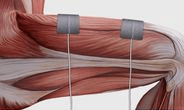
\includegraphics[width=\textwidth]{FES1.png}
		\caption{}
		\label{Figura: FES1}
	\end{subfigure}
	\hfill
	\begin{subfigure}[htbp]{0.4\textwidth}
		\centering
		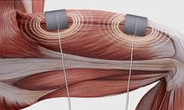
\includegraphics[width=\textwidth]{FES2.png}
		\caption{}
		\label{Figura: FES2}
	\end{subfigure}
	\caption[Efecto de aplicar estimulación eléctrica en músculo]{Efecto de aplicar estimulación eléctrica en músculo. (a) Músculo sin estimulación eléctrica. (b) Músculo con estimulación eléctrica. Recuperado de \cite{HASOMED}.}
	\label{Figura: FES}
\end{figure}

\section{Neuroprótesis}
Una neuroprótesis es un dispositivo compuesto de elementos que permiten utilizar la estimulación eléctrica como interface directa con el sistema nervioso, y cuyo fin es reemplazar o asistir alguna función deteriorada del sistema nervioso, deficiencia que suele ser el resultado de una enfermedad o lesión. Las neuroprótesis comúnmente actúan como un puente entre elementos funcionales del sistema nervioso central y los nervios o músculos sobre los cuales se ha perdido control (Figura \ref{Figura: NeuroP}) \cite{Finn2003}\cite{Popovic2008}.

En general, existen dos tipos de neuroprótesis: a) las neuroprótesis autónomas, las cuales son sistemas autocontenidos que imitan las funciones de una contraparte biológica, y b) las neuroprótesis por comando, las cuales son sistemas que reemplazan o asisten una función sensitiva o motora que se ha perdido o disminuido. Estas últimas están compuestos por un sistema de control que interpreta la intención del usuario, utilizan sensores para detectar el estado del sistema, genera la activación del sistema motor o sensorial del usuario, y proporciona una retroalimentación al usuario \cite{Popovic2015}.

Las neuroprótesis motoras, las cuales son un ejemplo de neuroprótesis por comando, son sistemas que asisten a personas que han sufrido algún tipo de lesión en la médula espinal o cerebro. Estas neuroprótesis pueden actuar directamente en el sistema nervioso central, en el sistema nervioso periférico, o bien, en una combinación de ambos, tiendo como objetivo principal realizar contracciones musculares que generen movimientos relevantes para el sujeto \cite{Popovic2015}.

%Figura Neuroprótesis
\begin{figure}[htbp]
	\centering
	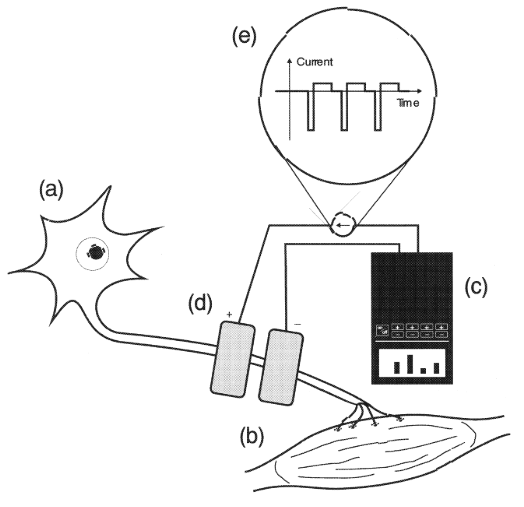
\includegraphics[width=0.4\textwidth]{NeuroP.png}
	\caption[Estimulación directa a una neurona motora]{Estimulación directa a una neurona motora. La neurona motora (a) es la responsable de generar señales de activación que son transmitidas a la correspondiente fibra muscular (b). Posterior a un accidente cerebrovascular o una lesión de la médula espinal, el músculo queda incomunicado con el sistema nervioso central. Una neuroprótesis (c) inyecta corriente eléctrica dentro del axón de la célula (d), corriente formada por un tren de pulsos negativos y positivos (e) que producen potenciales de acción que activan la fibra muscular. Recuperado de \cite{Popovic2008}.}
	\label{Figura: NeuroP}
\end{figure}

\section{Señales de comando y retroalimentación}\label{Seccion: ComRetro}

Una neuroprótesis por comando requiere de dos tipos de señales esenciales para lograr su correcto funcionamiento, las cuales son las señales de comando y las señales de retroalimentación \cite{Popovic2015}. En la Figura \ref{Figura: CompNeuroP} se pueden observar de forma general las conexiones que dichas señales realizan con el resto de los componentes de una neuroprótesis.

\begin{figure}[htbp]
\centering
	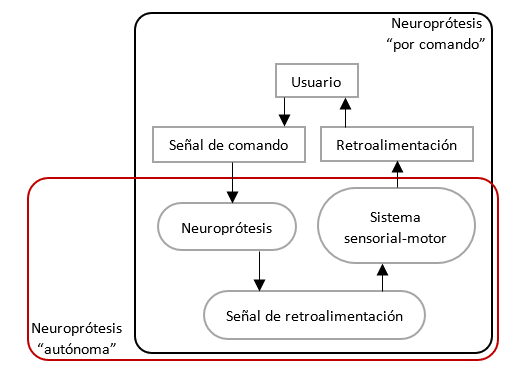
\includegraphics[width=0.6\textwidth]{CompNeuroP_ESP.png}
	\caption[Componentes generales de una neuroprótesis]{Componentes generales de una neuroprótesis autónoma (recuadro rojo) y por comando (recuadro negro). Adaptado de \cite{Popovic2015}.}
	\label{Figura: CompNeuroP}
\end{figure}

%\subsection{Señal de comando}
Las señales de comando son aquellas se usan para activar, desactivar o modular determinadas funciones o acciones dentro del sistema de control de la neuroprótesis. Estas señales pueden generarse de diversas formas, sin embargo, como se ilustra en la Figura \ref{Figura: CompNeuroP}, suelen ser generadas por el usuario \cite{Popovic2015}. Ejemplos de dichas señales podrían ser la acción de presionar un botón que indique a la neuroprótesis el momento de inicio y fin de la estimulación eléctrica; o bien, un conjunto de señales fisiológicas que permitan identificar la tarea que busca realizar el individuo.

%\subsection{Señal de retroalimentación}
En la Figura \ref{Figura: CompNeuroP} se puede observar que la señal de retroalimentación es aquella señal que se genera como salida de la neuroprótesis, es decir, la estimulación eléctrica que se inyecta al sistema sensorial-motor del usuario; sin embargo, también se puede observar una retroalimentación dirigida hacia el usuario, la cual hace referencia a la retroalimentación propioceptiva \cite{Popovic2015}. Esta última retroalimentación es la que suele ser relevante para el sistema de control de la neurorótesis.

Aclarado el concepto de retroalimentación que se abordará en el presente trabajo, se puede definir a las señales de retroalimentación como un tipo de señales que brindan información relacionada a la respuesta del sujeto ante un determinado comando. Dichas señales son útiles para indicar al sistema de control si la respuesta del sujeto se apega a la respuesta esperada, y en caso contrario modificar los parámetros de dicho sistema para conseguir la respuesta esperada \cite{Wright2016}. Estas señales de retroalimentación se pueden obtener de diversas maneras, las cuales se abordan en la sección \ref{Seccion: Retro}.

\section{Esquemas de control}
Existen dos tipos de control importantes dentro de las aplicaciones de una neuroprótesis, los cuales se diferencian esencialmente en los tipos de señales que ocupan. En la Figura \ref{Figura: EsqCont} se ilustran a grandes rasgos las diferencias entre ambos esquemas de control.

\begin{figure}[htbp]
\centering
	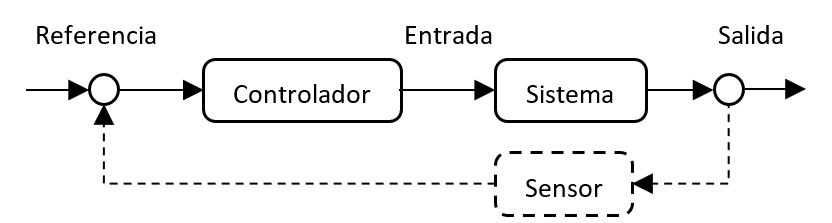
\includegraphics[scale=0.7]{EsquemasControl_ESP.png}
	\caption[Esquema general de control en lazo abierto y control en lazo cerrado]{Esquema general de control en lazo abierto y control en lazo cerrado. El control en lazo abierto se ilustra con una línea sólida. El control en lazo cerrado se lleva a cabo cuando se incluye el elemento sensor, el cual se ilustra con una línea discontinua. Adaptado de \cite{Wright2016}.}
	\label{Figura: EsqCont}
\end{figure}

%\subsection{Control en lazo abierto}
En el control en lazo abierto (línea sólida de la Figura \ref{Figura: EsqCont}) se genera un comando a la línea de base (estado o valor inicial del sistema), esperando que este comando produzca la salida correcta. Aquí no existe una medición de la salida generada, por lo cual tampoco existe alguna medición del error que pudiera utilizarse como mecanismo para la modulación del comando que se genera \cite{Wright2016}. En este esquema de control, los parámetros del sistema se encuentran predeterminados en base a consideraciones previas al experimento, y no sufren cambios durante la secuencia de estimulación.

%\subsection{Control en lazo cerrado}
El control en lazo cerrado (línea sólida más línea discontinua de la Figura \ref{Figura: EsqCont}) requiere de la inclusión de algún elemento sensor en el sistema que se desea controlar. Este control retroalimentado genera un comando a la línea de base y el elemento sensor mide la salida del sistema en respuesta al comando. Esta medición de la salida puede utilizarse para determinar diferencias entre la salida esperada y la real, generando así una señal de error que puede utilizarse como retroalimentación hacia el controlador para realizar modificaciones en los comandos generados \cite{Wright2016}.

%\subsection{Control adaptativo}
Otro esquema de control capaz de implementarse en aplicaciones de neuroprótesis (tanto en lazo abierto como en lazo cerrado) es el control adaptativo. Este esquema de control utiliza sensores para medir la entrada y salida del sistema, utilizando dichas métricas para ajustar el controlador en respuesta a las perturbaciones en el entorno de control o el sistema controlado, buscando siempre mantener un nivel de desempeño preestablecido. Una ventaja de este tipo de control es que se pueden desarrollar estrategias de control sin requerir de un conocimiento completo del sistema que se va a controlar, sin embargo, esto provoca que los controladores adaptativos rara vez sean óptimos \cite{Wright2016}.

\section{Algoritmos de control}
Existe una gran variedad de algoritmos de control que suelen ser usados dentro de las neuroprótesis, sin embargo, para este trabajo sólo se abordaran 3 algoritmos de control.

%\subsection{Control on-off}
El control on-off es un algoritmo que monitorea si una determinada variable de control se encuentra por encima o por debajo de un determinado umbral, con lo cual se suelen activar o desactivar determinadas funciones del sistema de control \cite{Wright2016}. En aplicaciones FES, este tipo de control suele utilizarse para activar una secuencia predefinida de estimulación eléctrica. Este algoritmo de control también suele utilizarse configurando dos umbrales por los cuales la variable de control puede pasar, por ejemplo, para el control de temperatura de una incubadora neonatal, en la cual se requiere que la temperatura de esta se encuentre dentro de un intervalo específico, en este caso, el control on-off podría aplicarse de la siguiente manera: si la temperatura se encuentra por encima del límite superior de temperatura, la calefacción se apaga; mientras que si la temperatura se encuentra por debajo del límite inferior de temperatura, la calefacción se enciende \cite{Wayne2003}.

%\subsection{Máquina de estados finitos (FSM)}
Una máquina de estados finitos (FSM, por sus siglas en inglés) es un modelo de sistema que puede considerarse como una implementación más compleja del control on-off. En este modelo, la medición de una variable del sistema en combinación con el estado actual de la misma, desencadenan una transición de estado, la cual a su vez genera una serie de acciones en el sistema que se está controlando. Debido a que este tipo de modelo suele ser periódico, puede ser útil para realizar transiciones de estado en respuesta al tiempo \cite{Wright2016}. En aplicaciones FES, las acciones generadas debido a la transición de estados suelen asociar al inicio o fin de la estimulación eléctrica, los periodos de rampa en el patrón de estimulación, o bien los periodos de modulación de la estimulación eléctrica.

%\subsection{Control proporcional}
El control proporcional (también conocido como control P), es un tipo control en el cual se aplica una corrección a la variable de control, la cual es proporcional entre el valor deseado y el valor real. Este tipo de control es más complejo que el control on-off, pero a su vez es más simple que un control proporcional-integral-derivativo (PID). Este tipo de control suele ser útil para llevar a cabo el control de sistemas que cuentan con un tiempo de respuesta rápido. En este tipo de control, la salida es proporcional a la señal de error (diferencia entre el valor esperado y el real), proporción que está definida por la Ecuación \ref{Ecu: Recta}, donde $P$ representa la salida proporcional, $K_{p}$ representa la ganancia proporcional, $e(t)$ representa el error instantaneo en el momento $t$, $p_{0}$ representa la salida con cero errores \cite{Wayne2003}. En aplicaciones FES, este tipo de control se ha mostrado útil para llevar a cabo la modulación de algún parámetro de estimulación eléctrica (como puede ser la amplitud o el ancho de pulso), donde la determinación de los factores $K_{p}$ y $p_{0}$ serán los responsables directos del grado de desempeño de la modulación \cite{Zhou2018}.

\begin{equation}
	P = K_{p} e(t) + p_{0}
	\label{Ecu: Recta}
\end{equation}

\section{Retroalimentación}\label{Seccion: Retro}
Como se explicó en la sección \ref{Seccion: ComRetro}, una señal de retroalimentación es aquella que brinda información al sistema sobre los efectos ante un determinado comando. Estas señales se pueden implementar de más de una forma dentro de una neuroprótesis, por ejemplo, la observación visual de la acción realizado por algún actuador robótico de una una interfaz cerebro-computadora (comúnmente conocido como neurofeedback), la adquisición de una señal bioeléctrica durante un periodo de estimulación eléctrica, o bien la medición de algún elemento sensor que proporcione información sobre el estado del efector o actuador \cite{Wright2016}.

Otro ejemplo de retroalimentación en un sistema de neuroprótesis es el biofeedback, una técnica de retroalimentación donde no se requiere de elemento sensor en el efector o actuador del sistema, ya que consiste en permitir al individuo usuario de la neuroprótesis aprender a cambiar su actividad fisiológica con el fin de mejorar el rendimiento del sistema \cite{Yucha2008}.

\section{Electromiografía de superficie}
La electromiografía (EMG) es una técnica electrofisiológica mediante la cual se registra la señal eléctrica derivada de la actividad contráctil de los músculos. El EMG puede detectarse directamente mediante la inserción de electrodos en las fibras musculares, o de forma indirecta colocando electrodos de superficie en las zonas de la piel localizadas justo encima del tejido muscular. A este último método se le suele conocer como electromiografía de superficie (sEMG, por sus siglas en inglés), el cual, al ser un método de detección no invasivo y permitir obtener información sobre la activación muscular, como la intensidad de la contracción muscular, la manifestación de la fatiga muscular y el reclutamiento de unidades motoras, se ha convertido en un método muy popular en la investigación.

\subsection{Procesamiento del sEMG}
La actividad mioeléctrica en la superficie de la piel se encuentra dentro de un ancho de banda limitado que suele estar desde los 15 hasta los 400 Hz, con amplitudes dentro del rango de $\mu V$ o $mV$, dependiendo de la intensidad de la contracción muscular \cite{Cavalcanti-Garcia2009}.

La detección de la actividad mioeléctrica se realiza mediante el uso de un amplificador diferencial, el cual debe tener conectadas las entradas a un par de electrodos situados a lo largo de la dirección de la fibra muscular a sensar, y un tercer electrodo de referencia situado en el hueso más cercano a la fibra. Una vez detectada de forma eficaz la actividad mioeléctrica, esta debe someterse a un filtro analógico anti-aliasing y posteriorme al proceso de conversión analógico-digital que permitirá se realice el procesamiento digital de la señal \cite{Cavalcanti-Garcia2009}.

Usualmente se utilizan técnicas de procesamiento digital, como un filtro pasa banda con frecuencias de corte similares a las que componen la actividad mioeléctrica (15-400 Hz), acompañado de un filtro notch que permita atenuar la interferencia provocada por la línea \cite{Cavalcanti-Garcia2009}.

\subsection{Descriptores de amplitud del sEMG}
Existen diferentes indicadores que pueden ser utilizados para estimar la amplitud del sEMG, tal es el caso de la amplitud pico a pico, la cual nos proporciona un valor instantáneo de la amplitud del sEMG. Sin embargo, este no es un indicador robusto de la amplitud de la señal de sEMG \cite{Cavalcanti-Garcia2009}.

Los descriptores de amplitud de sEMG más comunes son la promediación de muestras rectificadas o elevadas al cuadrado de sEMG crudo a lo largo de una determinada tarea motora. Estos descriptores se conocen como el valor rectificado promedio (ARV o MAV, por sus siglas en inglés)(Ecuación \ref{Ecu: ARV}) y el valor cuadrático medio (RMS, pos sus siglas en inglés)(Ecuación \ref{Ecu: RMS}). Dichos descriptores suelen usarse para estimar las variaciones temporales de la amplitud del sEMG en ventanas cortas entre 250 ms o 500 ms \cite{Cavalcanti-Garcia2009}.

\begin{equation}
	ARV = \frac{1}{N} \sum_{n=1}^{N} \abs{EMG[n]}
	\label{Ecu: ARV}
\end{equation}

\begin{equation}
	RMS = \sqrt{\frac{1}{N} \sum_{n=1}^{N} EMG[n]^{2}}
	\label{Ecu: RMS}
\end{equation}

Estos descriptores de amplitud suelen proporcionar información similiar, la gran diferencia entre ellos se encuentra en la función de densidad de probabilidad (PDF, por sus siglas en inglés) que generan, donde el RMS suele ser un descriptor con PDF Gaussiana, mientras que el ARV suele ser una descriptor con PDF Laplaciana. En general, se suele utilizar el RMS debido que teóricamente la PDF del sEMG es gaussiana, sin embargo, existen trabajos que han demostrado que en la práctica la PDF del sEMG es más cercana a una PDF laplaciana, en cuyo caso es recomendable utilizar el ARV como descriptor \cite{Clancy1999}\cite{Phinyomark2013}.

\chapter{Antecedentes}
\section{Desarrollos previos al proyecto}
En el INR-LGII se han realizado trabajos previos relacionados al desarrollo de una neuroprótesis, los cuales han logrado que dicho sistema sea funcional, e incluso se ha probado con algunos pacientes del propio instituto. Estos trabajos incluyen una plataforma de software para control y configuración de la neuroprótesis \cite{Fuentes2018}\cite{JanethFuentes2018} y la implementación de una aplicación FES en lazo abierto comandada por EEG\cite{Castillo2019}\cite{OmarCastillo2019}.

\subsection{Plataforma de software para neuroprótesis}
Consiste en una GUI implementada en MATLAB\textregistered \; (The MathWorks Inc., Natick, MA, E.U.A.), la cual consta de 4 pantallas que en conjunto permiten: a) realizar el registro de datos de un paciente o usuario en el que se probará el dispositivo, b) realizar el entrenamiento de un clasificador de movimientos voluntarios, c) ejecutar una aplicación FES en lazo abierto, o bien d) experimentar con los parámetros del estimulador y el sistema de registro de biopotenciales para determinar el patrón de estimulación óptimo para el paciente. Esta plataforma realiza una conexión a dispositivos comerciales: RehaStim 2 para estimulación eléctrica, y Cyton Board para adquisición de biopotenciales) que permiten la integración de las funciones de la neuroprotesis \cite{Fuentes2018}\cite{JanethFuentes2018}.

\subsection{Aplicación FES en lazo abierto}
La aplicación FES, que se encuentra inmersa en la plataforma de software para la neuroprótesis, está basada en una Interfaz Cerebro-Computadora. Dicha aplicación le muestra al sujeto una serie de 5 movimientos predefinidos, dentro de los cuales el sujeto debe seleccionar alguno cerrando los ojos. Una vez seleccionado y confirmado el movimiento objetivo, el sistema envía una secuencia de pulsos de estimulación eléctrica para asistir al sujeto a realizar el movimiento elegido. En esta aplicación los parámetros de estimulación eléctrica están predeterminados antes de iniciar la aplicación, los cuales se determinan en una sesión de calibración personalizada \cite{Castillo2019}\cite{OmarCastillo2019}.


\section{Sistemas FES existentes}
En la literatura existe una diversidad de trabajos que implementan un lazo cerrado para aplicaciones FES, los cuales utilizan dispositivos de estimulación que varían entre dispositivos comerciales o prototipos, sin embargo, la revisión bibliográfica realizada para este proyecto se centró en trabajos que utilizan el dispositivo RehaStim como dispositivo de estimulación, y que además implementaran alguna aplicación para rehabilitación de miembro superior.

Trabajos como los documentados en \cite{Salchow2016} y \cite{Kim2015}, muestran la importancia de las aplicaciones que implementan una terapia por medio de un entrenamiento en espejo para facilitar la recuperación motora de miembros superiores e inferiores en pacientes con hemiplejia. Dicha importancia radica en lograr la ilusión de un movimiento sincrónico entre dos extremidades sanas, ilusión que ha demostrado puede promover la recuperación de la funcionalidad de la extremidad paralizada \cite{Deconinck2015}.

El trabajo documentado en \cite{Sun2014} demuestra la gran capacidad que tienen los algoritmos implementados en una máquina de estados finitos para realizar el control de una neuroprótesis, además de demostrar que estos algoritmos permiten al experimentador una comprensión rápida sobre el funcionamiento del esquema de control.

Otros trabajos como lo son \cite{Simonsen2017} y \cite{Woods2018} son de utilidad para el proyecto debido a que demuestran que al lograr una integración de los componentes y control de una neuroprótesis se pueden realizar aplicaciones que presenten un funcionamiento en tiempo real o muy cercano a este.

El Cuadro \ref{Cuadro:Sistemas FES} resume la información de los trabajos mencionados anteriormente, mostrando información como autor, año de publicación, propósito del trabajo, señales de comando y retroalimentación utilizadas, y dispositivo de estimulación. Cabe mencionar que todos estos trabajos presentan una implementación dentro de las plataformas de software MATLAB\textregistered \; y Simulink\textregistered.

%Cuadro de revisión bibliográfica
\begin{table}[hbt]
	\centering
	\begin{tabular}{|p{30mm}|p{10mm}|p{40mm}|p{40mm}|p{25mm}|}
	\hline
	\textbf{Autor} & \textbf{Año} & \textbf{Propósito} & \textbf{Señales utilizadas} & \textbf{Dispositivo}\\ 
	\hline
	\hline
	Christina Salchow, \emph{et al.} \cite{Salchow2016} & 2016 & Entrenamiento en espejo aplicado a la mano & Electromiografía y movimiento de mano & RehaMove Pro\\
	\hline
	Mignxu Sun \cite{Sun2014} & 2014 & Recuperación de funciones de miembro superior & Acelerometría & RehaStim 1\\
	\hline
	Daniel Simonsen, \emph{et al.} \cite{Simonsen2017} & 2017 & Asistencia para apertura y cierre de mano & Posición del objeto y posición de la mano & STMISOLA\\
	\hline
	Billy Woods, \emph{et al.} \cite{Woods2018} & 2018 & Asistencia en miembro inferior para funciones de ciclismo & Mecanomiografía, fuerza aplicada a pedales y posición de cigüeñal & RehaStim 1\\
	\hline
	\end{tabular}
	\caption{Revisión de sistemas FES reportados en la literatura con aplicaciones similares a las de este proyecto.}
	\label{Cuadro:Sistemas FES}
\end{table}

Una revisión bibliográfica adicional se centró en trabajos que utilizaran señales de sEMG como señal de control, para rescatar los descriptores de amplitud comúnmente usados y los tipos de control utilizados para cada aplicación.

El Cuadro \ref{Cuadro:Control} resumen la información de los trabajos consultados para dicha revisión bibliográfica, mostrando información como autor, año de publicación, propósito de la aplicación, descriptor de amplitud utilizado y tipo de control implementado.

\begin{table}[htb]
	\centering
	\begin{tabular}{|p{30mm}|p{10mm}|p{45mm}|p{25mm}|p{35mm}|}
	\hline
	\textbf{Autor} & \textbf{Año} & \textbf{Propósito} & \textbf{Descriptor sEMG} & \textbf{Tipo de control}\\
	\hline
	\hline
	Yu Zhou, \emph{et al.} \cite{Zhou2018} & 2018 & FES contralateral para miembro superior & RMS & Regresión lineal\\
	\hline
	Tommaso Lenzi, \emph{et al.} \cite{Lenzi2012} & 2012 & Control de exoesqueleto & Envolvente lineal & Proporcional\\
	\hline
	Jung Hee Kim, \emph{et al.} \cite{Kim2015} & 2015 & Terapia en espejo para recuperación de miembro superior & RMS & On-Off\\
	\hline
	Gustavo Aguirre, \emph{et al.} \cite{Aguirre-Vargas2015} & 2015 & Control de brazo robótico & Amplitud & Lógica difusa\\
	\hline
	Xin Yi, \emph{et al.} \cite{Yi2013} & 2013 & Cierre contralateral de párpado en conejos & RMS & On-Off\\
	\hline
	Sachs NA, \emph{et al.} \cite{Sachs2006} & 2006 & Cierre contralateral de párpado en roedores & Integración & On/Off\\
	\hline
	Lucas Fonseca, \emph{et al.} \cite{Fonseca2019} & 2019 & Asistencia contralateral para cierre de mano & Envolvente & FSM\\
	\hline
	\end{tabular}
	\caption{Revisión de tipos de control y descriptores de amplitud comúnmente usados en aplicaciones de control basado en sEMG.}
	\label{Cuadro:Control}
\end{table}


\chapter{Metodología}
\section{Sistema propuesto}
Para este proyecto se planteó un sistema que implementa un control de FES en lazo cerrado utilizando la técnica de biofeedback. El sistema consiste en la adquisición de dos canales de sEMG del brazo izquierdo, los cuales son procesados y se utilizan como entrada de un sistema de control que realiza la modulación de la amplitud de dos canales de estimulación eléctrica en el brazo derecho. Este sistema implementa un control contralateral para realizar un entrenamiento en espejo de las acciones de apertura de mano y pinza gruesa.

En la Figura \ref{Figura: SistProp} se muestra un esquema general del sistema desarrollado, en el cual se muestran en rojo los elementos implementados en este proyecto.

%Sistema propuesto
\begin{figure}[htbp]
\centering
	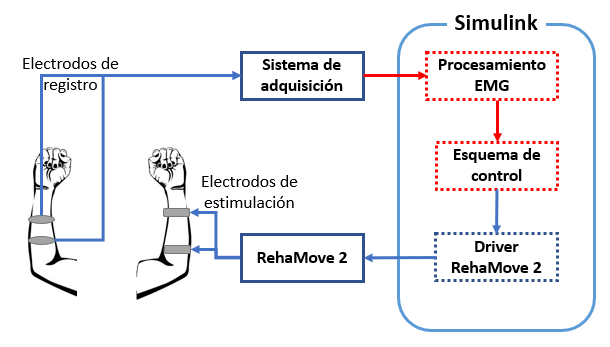
\includegraphics[scale=0.7]{SistemaPropuesto.png}
	\caption[Sistema propuesto para el proyecto]{Sistema propuesto para el proyecto. Líneas continuas representan entes de hardware y líneas discontinuas representan entes de software. Elementos en rojo representan zonas de trabajo de este.}
	\label{Figura: SistProp}
\end{figure}


\section{Adquisición de datos en Simulink\textregistered} \label{Sec: Adquisicion}
Para realizar la adquisición de las señales de sEMG se utilizó el sistema Cyton Board, el cual tiene una frecuencia de muestreo de 250 Hz. Dicho sistema utiliza un chip ADS1299 (Texas Instruments Inc., Dallas, E.U.A.) para realizar la conversión analógico-digital de las señales, el cual codifica los datos de cada muestra, utilizando codificación en complemento a 2, en un flujo de datos de 27 bytes en formato MSBF (most significant bit first) esquematizado en la Figura \ref{Figura: BusOut}. En dicha figura se aprecia claramente que cada muestra de cada canal está conformada por 3 bytes , formando un total de 24 bytes para los 8 canales, mientras que los primeros 3 bytes corresponden a información de estado propia del ADS1299.

%Stream datos ADS
\begin{figure}[htbp]
\centering
	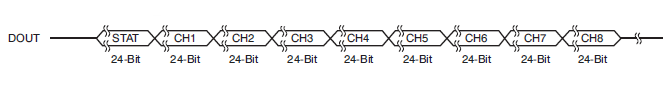
\includegraphics[scale=0.8]{Bus_Dat_Out_ADS.png}
	\caption{Flujo de datos de salida del ADS1299.}
	\label{Figura: BusOut}
\end{figure}

Para realizar la decodificación del flujo de datos dentro de Simulink\textregistered, se diseñó un subsistema encargado de la solicitud y decodificación de datos, para esto se utilizó el bloque \emph{Query Instrument} del \emph{Instrument Control Toolbox} para realizar la solicitud de datos, los cuales fueron decodificados con bloques de la librería estándar de Simulink\textregistered. La figura \ref{Figura: DecoSimuT} muestra la implementación de este subsistema.

\vfill
%Sistema Simulink
\begin{figure}[htbp]
	\centering
	\begin{subfigure}[htbp]{0.8\textwidth}
		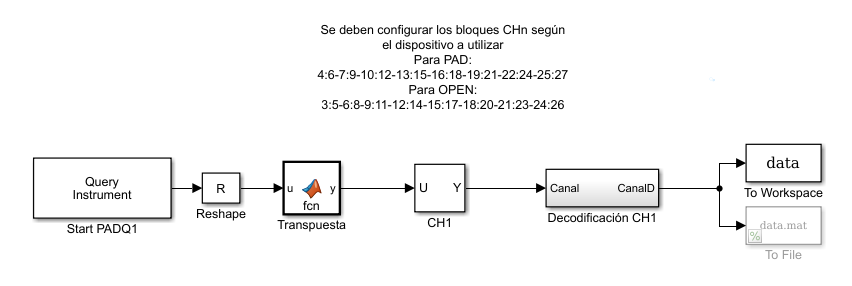
\includegraphics[width=\textwidth]{Read_Simu.png}
		\caption{}
		\label{Figura: readSimu}
	\end{subfigure}
	\begin{subfigure}[htbp]{0.75\textwidth}
		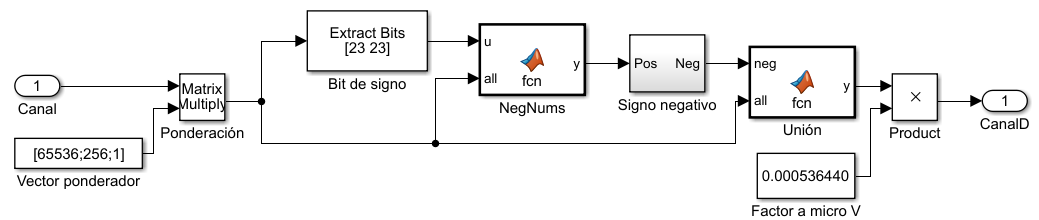
\includegraphics[width=\textwidth]{Deco_Simu.png}
		\caption{}
		\label{Figura: decoSimu}
	\end{subfigure}
	\caption[Diagrama de bloques del subsistema decodificador del flujo de datos]{Diagrama de bloques del subsistema decodificador del flujo de datos implementado en Simulink\textregistered . (a) Vista general del subsistema diseñado para realizar adquisición y decodificación del flujo de datos. (b) Vista interna del subsistema encargado de la decodificación del flujo de datos.}
	\label{Figura: DecoSimuT}
\end{figure}

\newpage
El funcionamiento del subsistema responsable de la solicitud y decodificación de datos implementado dentro de Simulink\textregistered \; se encuentra esquematizado en la Figura \ref{Figura: DecoStream}, y lleva a cabo el siguiente algoritmo:

\begin{enumerate}
	\item Se realiza la adquisición de N muestras, lo cual generará un vector columna con dimensión $(27*N)\times 1$ (Figura \ref{Figura: DecoStream} \emph{(a)}), donde 27 corresponde al tamaño en bytes del flujo de datos a recibir y 1 corresponde a 1 columna en la que se recibirán los datos.
	
	\item Se aplica una operación de reshape a dicho vector para obtener una matriz con dimensión $27\times N$ (Figura \ref{Figura: DecoStream} \emph{(b)}).
	
	\item Se obtiene la transpuesta de dicha matriz para obtener una matriz de dimension $N\times 27$ (Figura \ref{Figura: DecoStream} \emph{(c)}).
	
	\item Se realiza la extracción de las columnas asociadas al canal a procesar, obteniendo una matriz de dimensión $N\times 3$ (Figura \ref{Figura: DecoStream} \emph{(d)}), donde 3 es el número de bytes correspondientes a cada muestra.
	
	\item Se realiza el producto de la matriz del canal a procesar con un vector (columna) ponderador que contiene el peso de cada columna (byte) necesario para obtener el valor de la muestra de 24 bits (Figura \ref{Figura: DecoStream} \emph{(e)}). El vector ponderador está compuesto por los valores $2^{16}$, $2^8$ y $2^0$, los cuales corresponden a realizar un corrimiento hacia la izquierda de 16, 8 y 0 bits respectivamente. Como resultado de dicho producto se obtiene un vector de dimensión $N\times 1$ en unidades de bits (Figura \ref{Figura: DecoStream} \emph{(f)}).
	
	\item Se extraen del vector \emph{f} las muestras en las que se encuentren codificados, en complemento a 2, un número negativo. Esto se realiza al obtener el valor del bit 23 (bit más significativo), y si dicho bit tiene un valor de 1 implica que dicha muestra codifica un número negativo. De esta operación se obtiene un vector con dimensión $M\times 1$, donde $M$ es la cantidad de muestras negativas a decodificar. (Figura \ref{Figura: DecoStream} \emph{(g)}).
	
	\item Se obtiene el complemento a 1 de cada elementro (muestra) del vector \emph{g}, sumando 1 a cada muestra y multiplicándola por -1. De esta operación se obtiene un vector con las muestras decodificadas a número binarios con signo negativo (Figura \ref{Figura: DecoStream} \emph{(h)}).
	
	\item Se insertan los elementos del vector \emph{h} en sus posiciones originales del vector \emph{f}. De este último paso se obtiene un vector con las N muestras decodificadas a números de 24 bits con signo en unidades de bits (Figura \ref{Figura: DecoStream} \emph{(i)}).
	
	\item Por último, para  obtener unidades de voltaje, se multiplica cada elemento del vector \emph{i} por un factor de escalamiento determinado por la Ecuación \ref{Ecu: ScaleFactor}. Obteniendo como resultado un vector columna con las N muestras adquiridas en unidades de voltaje e incluyen el valor de la ganancia.
\end{enumerate}

\vfill
\begin{equation}
	Factor\; de\; Escalamiento = V_{ref}/(2^{23}-1)
	\label{Ecu: ScaleFactor}
\end{equation}
\vfill

%Funcionamiento decodificación
\begin{figure}[htbb]
\centering
	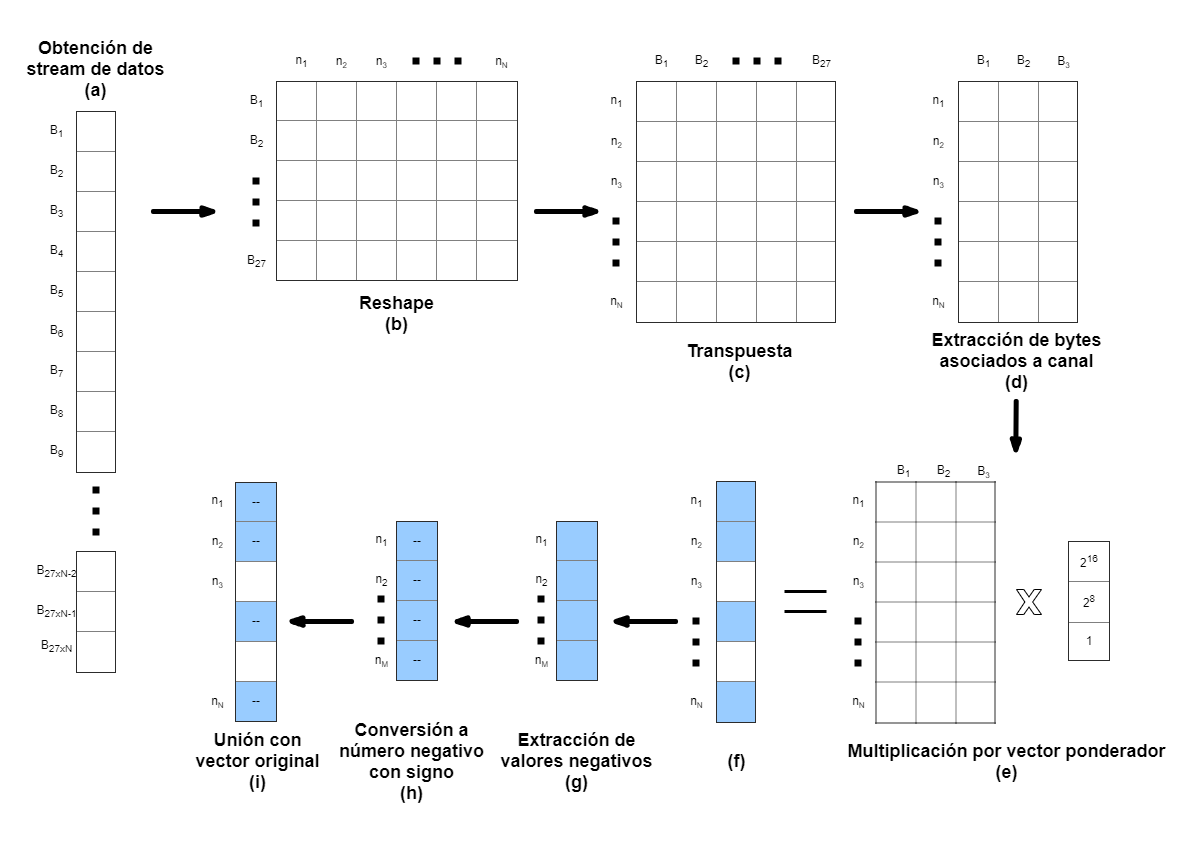
\includegraphics[width=\textwidth]{DecoStream.png}
	\caption{Funcionamiento del subsistema decodificador del flujo de datos.}
	\label{Figura: DecoStream}
\end{figure}
\vfill

\newpage
\section{Evaluación de bloque de adquisición y decodificación}\label{Sec: EvalAdquisicion}
Se llevó a cabo un procedimiento para evaluar el desempeño del subsistema diseñado en Simulink\textregistered \; para la adquisición y decodificación de datos. En MATLAB\textregistered \; se generó un banco de señales senoidales conformado por 5 senoidales puras de 1 Hz, 5 Hz, 10 Hz, 20 Hz, 50 Hz y 100 Hz (Figura \ref{Figura: SenPur}), tres senoidales de 50 Hz moduladas en amplitud con distintas envolventes: 
una envolvente de una recta con pendiente negativa (Figura \ref{Figura: LinAte}), una envolvente de una exponencial decreciente (Figura \ref{Figura: ExpAte}), y una envolvente que simula la señal sEMG correspondiente a la tarea de incrementar gradualmente una contracción muscular, mantener dicha contracción y relajar el músculo gradualmente (Figura \ref{Figura: Contra}). Todas las señales del banco se diseñaron con una frecuencia de muestreo de 250 Hz y una duración de 5 segundos, excepto la última, que se diseñó con una duración de 15 segundos; adicionalmente, todas las señales se generaron como objetos de audio dentro de MATLAB\textregistered, para poder reproducirlas como audio y a partir de la salida de audio de la computadora poder acceder a ellas.

%Figura de senoidales MATLAB
\begin{figure}[htbp]
	\centering
	\begin{subfigure}[htbp]{0.45\textwidth}
		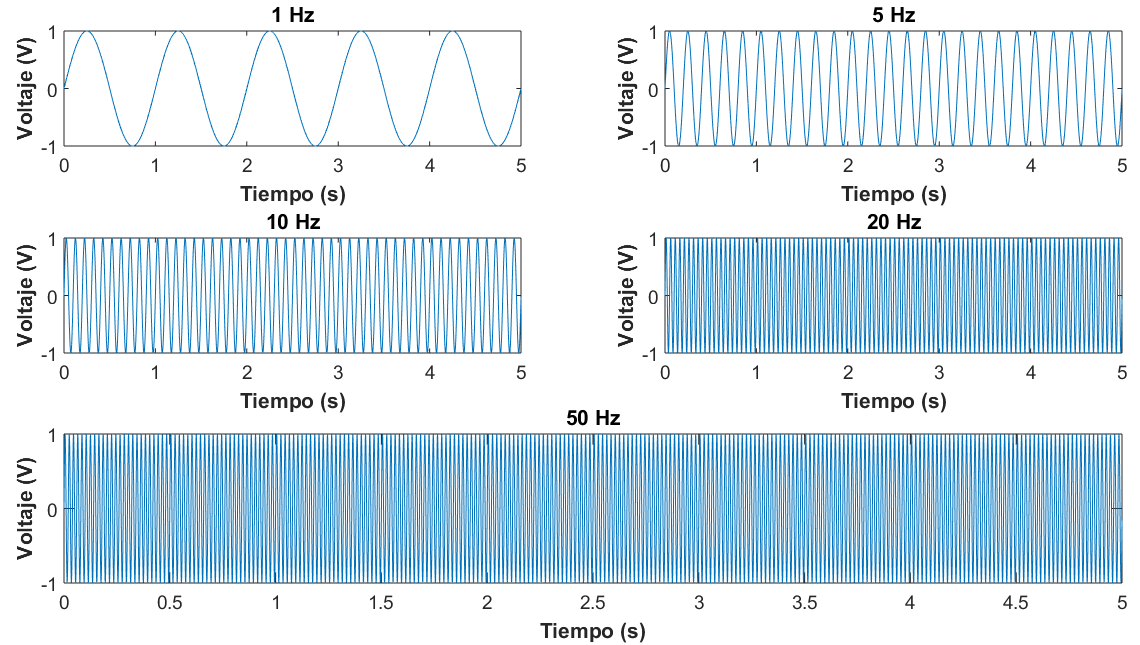
\includegraphics[width=\textwidth]{Sen_Pur.png}
		\caption{}
		\label{Figura: SenPur}
	\end{subfigure}
	\hfill
	\begin{subfigure}[htbp]{0.45\textwidth}
		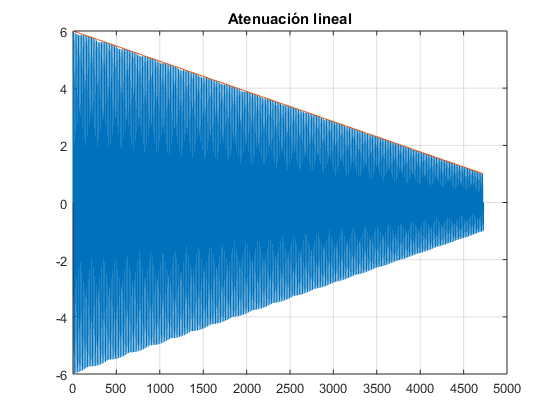
\includegraphics[width=\textwidth]{Lin_Ate.png}
		\caption{}
		\label{Figura: LinAte}
	\end{subfigure}
	\hfill
	\begin{subfigure}[htbp]{0.45\textwidth}
		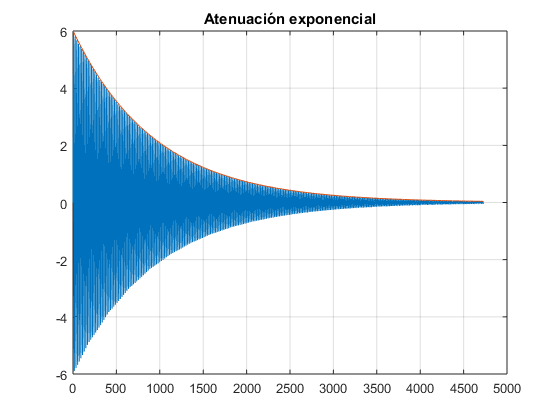
\includegraphics[width=\textwidth]{Exp_Ate.png}
		\caption{}
		\label{Figura: ExpAte}
	\end{subfigure}
	\hfill
	\begin{subfigure}[htbp]{0.45\textwidth}
		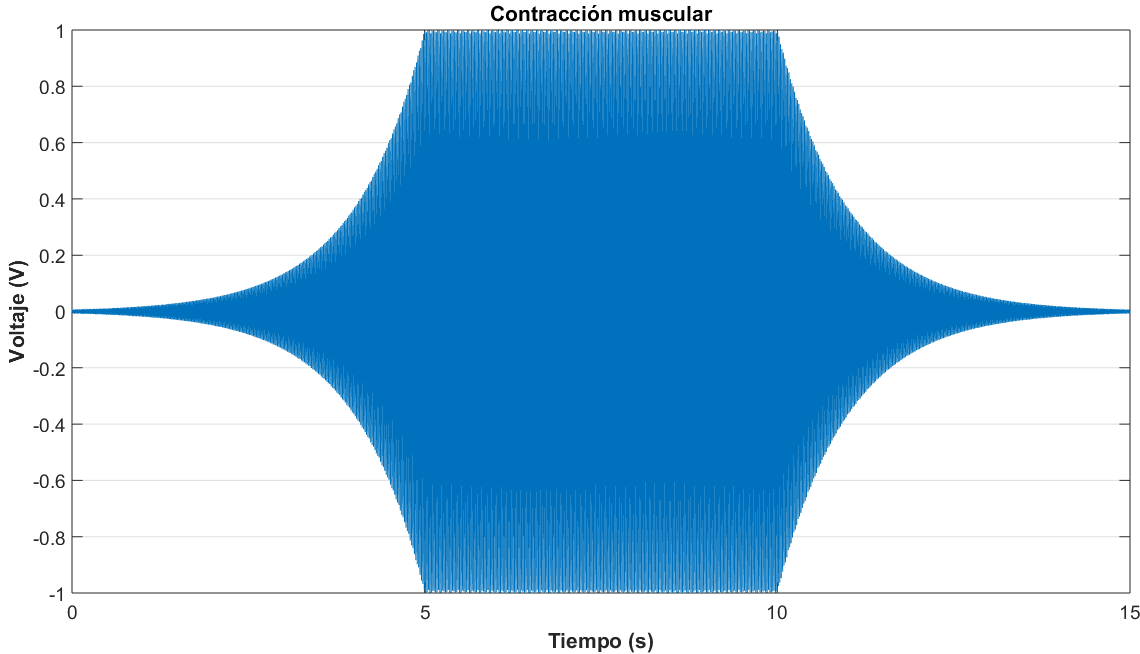
\includegraphics[width=\textwidth]{Contra.png}
		\caption{}
		\label{Figura: Contra}
	\end{subfigure}	
	\caption[Banco de señales para evaluación de adquisición]{Banco de señales para evaluación de adquisición. (a) Senoidales puras a diferentes frecuencias. (b) Senoidal de 50 Hz con atenuación lineal. (c) Senoidal de 50 Hz con atenuación exponencial. (d) Senoidal de 50 Hz simulando el sEMG de una contracción muscular.}
	\label{Figura: SenalesEva}
\end{figure}

\newpage
El proceso para la evaluación del funcionamiento del subsistema de adquisición se llevó a cabo de la siguiente manera:
\begin{enumerate}
	\item Se realiza la adquisición de tres repeticiones de cada una de las señales del banco de señales de prueba.
	\begin{enumerate}
		\item Se conecta una punta de un jack de audio de 3.5 mm a la salida de audio de la computadora. La otra punta se conectó al dispositivo de adquisición (Cyton Board) de la siguiente forma: el pin \emph{izquierdo} se conectó a un pin diferencial del canal 1, mientras que el pin \emph{tierra} se conectó a la entrada BIAS y al pin diferencial restante del canal 1. La Figura \ref{Figura: JackConexion} ilustra estas conexiones.
		\item Se realiza la solicitud de datos utilizando el subsistema decodificador implementado en Simulink\textregistered \; (Figura \ref{Figura: DecoSimuT}), y al mismo tiempo se inicia el conteo de un cronómetro.
		\item Dos segundos después de haber iniciado la solicitud de datos, se procede a reproducir la señal de audio de prueba.
		\item Tras haber transcurrido 10 s (20 s para la simulación del sEMG de una contracción), se detiene la adquisición del subsistema de Simulink\textregistered \; y se guardan los datos registrados dentro de un archivo con extensión \emph{.mat}.
	\end{enumerate}
	\item Se cargan, dentro del workspace de MATLAB\textregistered, los datos de las señales adquiridas y los datos de las señales patrón.
	\item Se procede a alinear de forma manual la señal adquirida con la señal patrón, y posteriormente se calcula el coeficiente de correlación de Pearson (Ecuación \ref{Ecu: CorrePea}. Donde $\sigma_{xy}$ representa la covarianza de $x$,$y$; $\sigma_{x}$ representa la desviación estándar de $x$; y $\sigma_{y}$ representa la desviación estándar de $y$) entre ambas señales.
	\item Se obtiene la media aritmética de los valores obtenidos al aplicar el coeficiente de correlación de Pearson a cada una de las señales registradas (24 registros en total). El valor obtenido se utiliza como indicador de la calidad del subsistema de adquisición y decodificación de datos.
\end{enumerate}

\vfill
%Ecuación correlación Pearson
\begin{equation}
	r = \frac{\sigma_{xy}}{\sigma_{x}\sigma_{y}}
	\label{Ecu: CorrePea}
\end{equation}
\vfill

\begin{figure}
	\centering
	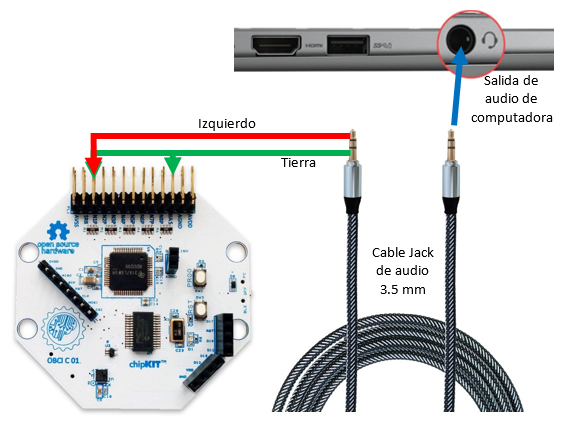
\includegraphics[width=0.5\textwidth]{JackConexion.png}
	\caption{Conexiones para evaluación de bloque de adquisición.}
	\label{Figura: JackConexion}
\end{figure}

\newpage
\section{Protocolo para registro de sEMG}\label{Sec: ProReg}
Para garantizar repetibilidad en los registros de sEMG se implementó un protocolo para realizar la adquisición de dicha señal. Dicho protocolo se describe a continuación y utiliza electrodos Telectrode T718 (Bio-Protech Inc., Chino, E.U.A.):

\begin{enumerate}
	\item Se configura el dispositivo de adquisición (Para el caso del Cyton Board esta configuración es la preprogramada por el fabricante):
	\begin{enumerate}
		\item Frecuencia de muestreo a 250 Hz.
		\item Ganancia 24 para los canales de adquisición 1 y 2.
	\end{enumerate}
	\item Se preparan las zonas donde se colocaran los electrodos para registro de sEMG, limpiando con algodón y alcohol las zonas ventral y dorsal del antebrazo, así como el codo.
	\item Se ubican los puntos para colocación de electrodos:
	\begin{enumerate}
		\item Para el par de electrodos que registrará la actividad relacionada con el movimiento de flexión de dedos (pinza gruesa), el músculo asociado es el músculo flexor digitorum (Figura \ref{Figura: E_Cie}):
		\begin{enumerate}
			\item Se mide la distancia de codo a muñeca en el lado ventral del antebrazo.
			\item Se coloca una marca al 25\% de la medida obtenida.
		\end{enumerate}
		\item Para el par de electrodos que registrará la actividad relacionada con el movimiento de extensión de dedos (apertura de mano), el músculo asociado es el músculo extensor digitorum (Figura \ref{Figura: E_Ape}):
		\begin{enumerate}
			\item Se mide la distancia de codo a muñeca en el lado dorsal del antebrazo.
			\item Se coloca una marca al 75\% de la medida obtenida.
		\end{enumerate}
	\end{enumerate}
	\item Se colocan, centrados sobre la marca obtenida para el flexor digitorum (Figura \ref{Figura: E_Cie}), dos electrodos (en dirección de las fibras musculares) separados 3 cm. Este par de electrodos se conecta al canal 1 del dispositivo de adquisición por medio de cables con conector tipo Snap.
	\item Se colocan, centrados sobre la marca obtenida para el extensor digitorum (Figura \ref{Figura: E_Ape}), dos electrodos (en dirección de las fibras musculares) separados 3 cm. Este para de electrodos se conecta al canal 2 del dispositivo de adquisición por medio de cables con conector tipo Snap.
	\item Se coloca un electrodo de referencia sobre el codo. Dicho electrodo se conecta al pin BIAS del dispositivo de adquisición.
\end{enumerate}

\vfill
%Ubicación electrodos
\begin{figure}[htbp]
	\centering
	\begin{subfigure}[htbp]{0.3\textwidth}
		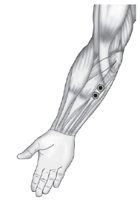
\includegraphics[width=\textwidth]{E_Cie.png}
		\caption{}
		\label{Figura: E_Cie}
	\end{subfigure}
%	\hfill
	\hspace{3cm}
	\begin{subfigure}[htbp]{0.3\textwidth}
		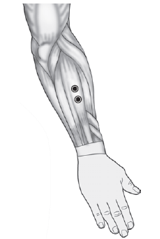
\includegraphics[width=\textwidth]{E_Ape.png}
		\caption{}
		\label{Figura: E_Ape}
	\end{subfigure}
	\caption[Posicionamiento de electrodos para registro de sEMG]{Posicionamiento de electrodos para registro de sEMG. Adaptado de \cite{Cavalcanti-Garcia2009}. (a) Ubicación de electrodos para flexor digitorum. (b) Ubicación de electrodos para extensor digitorum.}
	\label{Figura: E_sEMG}
\end{figure}
\vfill

\newpage
\section{Procesamiento de sEMG} \label{Sec: Procesamiento}
Se diseñaron tres filtros digitales Butterworth de orden 2 para realizar el procesamiento de sEMG:

\begin{itemize}
	\item Un filtro pasa altas con frecuencia de corte de 15 Hz, para eliminar las variaciones en la línea base del registro.
	\item Un filtro pasa bajas con frecuencia de corte de 100 Hz, para eliminar armónicos de 60 Hz y demás interferencias de alta frecuencia.
	\item Un filtro rechaza banda centrado en 60 Hz, para reducir la interferencia de la línea.
\end{itemize}

Todos estos filtros se diseñaron utilizando la función \emph{butter} de MATLAB\textregistered. Las gráficas de respuesta en frecuencia de estos filtros se muestran en la Figura \ref{Figura: Freqz_Filtros} 

%Respuesta en frecuencia de filtros
\begin{figure}[htbp]
	\centering
	\begin{subfigure}[htbp]{0.7\textwidth}
		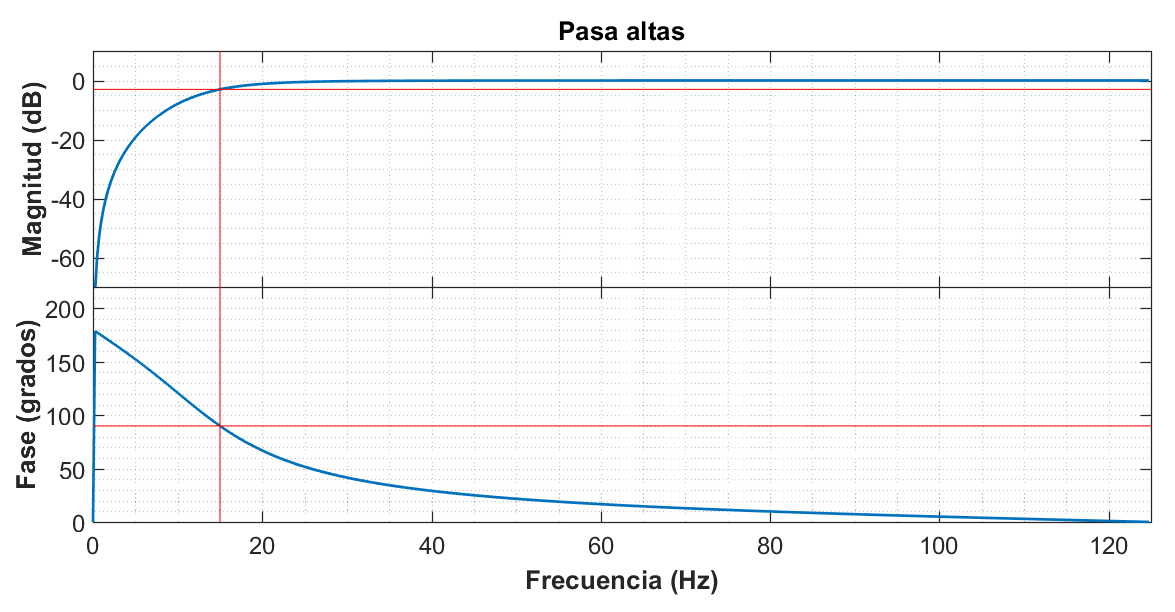
\includegraphics[width=\textwidth]{FiltroPA15Hz_PADQ.png}
		\caption{}
		\label{Figura: FiltroPA}
	\end{subfigure}
	
	\begin{subfigure}[htnp]{0.7\textwidth}
		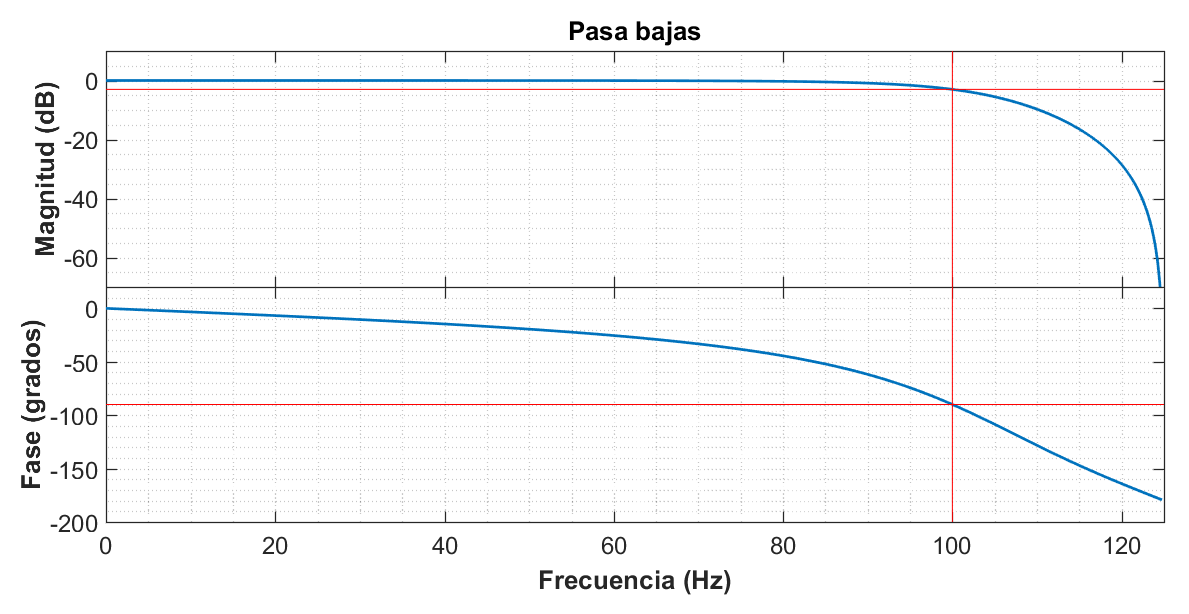
\includegraphics[width=\textwidth]{FiltroPB100Hz_PADQ.png}
		\caption{}
		\label{Figura: FiltroPB}
	\end{subfigure}
	
	\begin{subfigure}[htbp]{0.7\textwidth}
		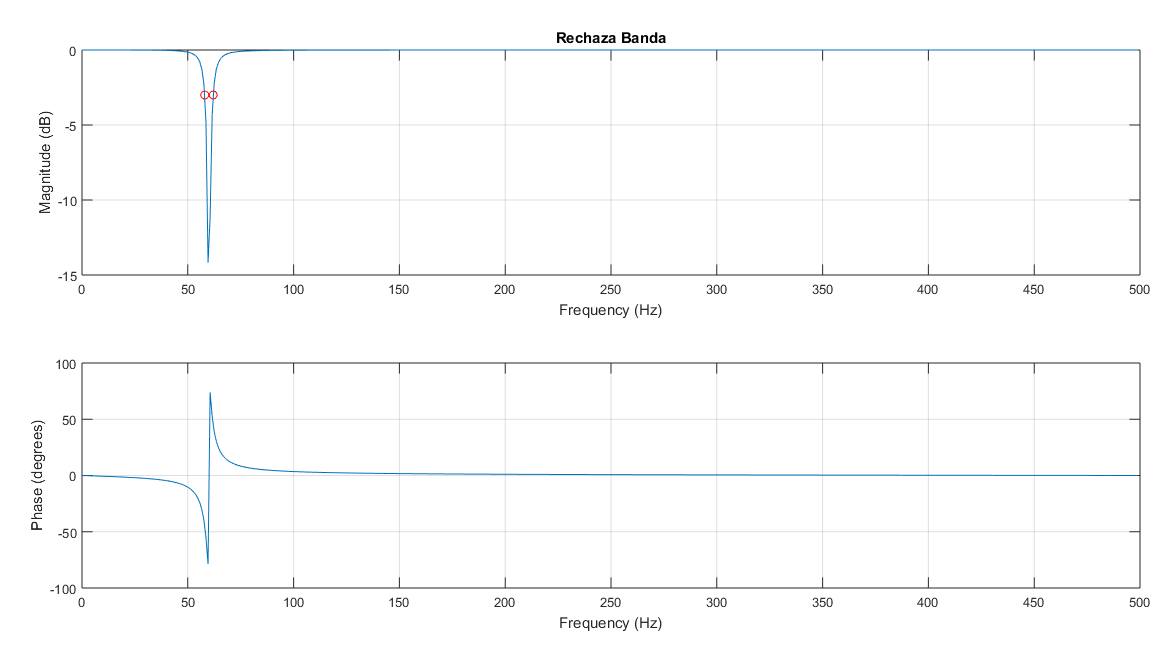
\includegraphics[width=\textwidth]{FiltroRB_58_62_PADQ.png}
		\caption{}
		\label{Figura: FiltroRB}
	\end{subfigure}
	\caption[Respuesta en frecuencia del banco de filtros diseñado]{Respuesta en frecuencia del banco de filtros diseñado. (a) Filtro pasa altas. (b) Filtro pasa bajas. (c) Filtro rechaza banda.}
	\label{Figura: Freqz_Filtros}
\end{figure}

Se implementó dentro de Simulink\textregistered \;un bloque responsable de obtener el valor RMS de ventanas de 100 ms (25 muestras para una frecuencia de muestro de 250 Hz) del registro de sEMG, para utilizar dicho descriptor de amplitud como señal de control. Adicionalmente se implementó un filtro de mediana de 10 muestras, el cual tiene como propósito conseguir una señal RMS suavizada. La Ecuación \ref{Ecu: Mediana} describe al filtro de mediana, donde $x$ representa la señal RMS a suavizar, $n$ representa la n-ésima muestra de dicha señal, $N$ representa la cantidad de muestras del filtro (en este caso 10), mientras que $y$ representa el valor de la señal RMS suavizada.

%Ecuación filtro mediana
\begin{equation}
	y[n] = mediana(x[n]:x[n-N])
	\label{Ecu: Mediana}
\end{equation}


\newpage
\section{Sistema de control}
A grandes rasgos, el sistema de control implementado para este proyecto consta de la combinación de una FSM y un mapeo proporcional. La FSM (Figura \ref{Figura: FSM_Control})  determina el canal de estimulación eléctrica que se activará, a partir de la salida del algoritmo para la detección de movimiento, el cual clasifica la intención de movimiento del sujeto en tres clases (descanso, pinza gruesa y apertura de mano), mientras que el mapeo proporcional permite realizar la modulación de la amplitud de corriente eléctrica a partir de la amplitud del sEMG.

%FSM
\begin{figure}[htbp]
	\centering
	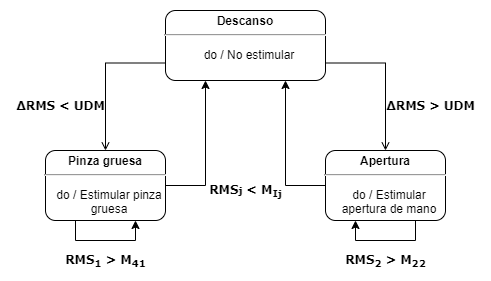
\includegraphics[scale=0.7]{FSM_Control.png}
	\caption[FSM para control]{Máquina de estados finitos encargada de la detección de movimiento e inicio del control proporcional.}
	\label{Figura: FSM_Control}
\end{figure}

La máquina de estados necesita principalmente tres parámetros para llevar a cabo la transición entre los movimientos: umbral detector de movimiento ($UDM$), umbral de pinza gruesa incompleta ($M_{41}$) y umbral de apertura de mano incompleta ($M_{22}$). Dentro de los estados pinza gruesa y apertura de mano, la FSM necesita de una ecuación de mapeo proporcional para poder llevar a cabo la modulación de la estimulación eléctrica. La obtención de dichos parámetros se obtiene de un proceso de calibración que se realiza para cada sesión de prueba.

Posterior al proceso de calibración se realiza una validación fuera de línea, donde a partir del registro de calibración y los parámetros arrojados por esta se pone a prueba el funcionamiento del sistema. Cuando la validación fuera de línea presenta un porcentaje de acierto igual o mayor al 80$\%$ se procede a configurar el sistema para realizar una prueba en línea y posteriormente realizar la tarea objetivo.

Todas las etapas antes mencionadas del sistema de control y sus componentes se describen a continuación.

\subsection{Calibración}\label{Sec: Calibracion}
El proceso de calibración del sistema se divide en una calibración de los parámetros de estimulación eléctrica y una calibración de los valores de amplitud RMS del sEMG.

\subsubsection{Calibración de parámetros FES}\label{Sec:CalFES}
El objetivo de esta calibración es el obtener los umbrales motores y funcionales de los movimientos de apertura de mano y pinza gruesa. Para esta calibración se utiliza el sistema de colocación de electrodos de estimulación eléctrica desarrollado en el INR-LGII, el cual se encuentra descrito en \cite{AnaMartin2019}, en conjunto con la pantalla \emph{Experimentación} (Figura \ref{Figura: GUI_Exp}) de la GUI diseñada en el INR-LGII \cite{JanethFuentes2018}.

El proceso para la obtención de los umbrales antes mencionados consiste en realizar la colocación de los electrodos de estimulación eléctrica para los movimientos objetivo (que en este caso son los movimientos de pinza gruesa y apertura de mano) y realizar una exploración de la respuesta del sujeto ante diferentes valores de amplitud de corriente eléctrica que le serán proporcionados. Dichos valores exploran el rango entre 1 y 15 mA, utilizando un incremento de 1 mA. El umbral motor será el primer valor de amplitud que genere una respuesta motora notable a simple vista y reconocida por el sujeto en la mano del sujeto; mientras que el umbral funcional será aquél valor de amplitud que provoque el movimiento objetivo de la mano con un rango de movimiento completo, similar a un movimiento voluntario

%Experimentación
\begin{figure}[htb]
	\centering
	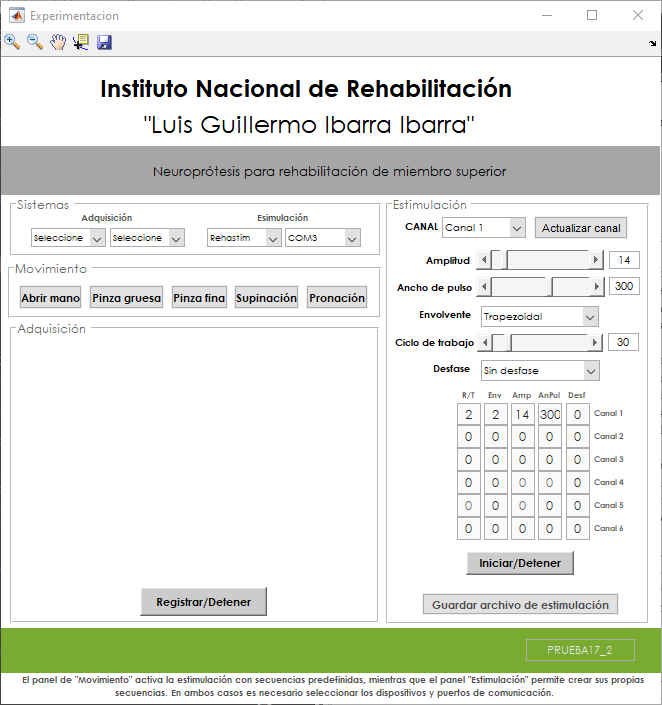
\includegraphics[width=0.6\textwidth]{GUI_Exp.png}
	\caption{GUI utilizada para calibración de FES.}
	\label{Figura: GUI_Exp}
\end{figure}

\subsubsection{Calibración de umbrales RMS de sEMG}\label{Sec:CalRMS}
Para realizar esta calibración se utiliza el protocolo de registro descrito en la sección \ref{Sec: ProReg} y una pantalla de calibración diseñada para este proyecto (Figura \ref{Figura: GUI_Ent}), la cual muestra indicaciones en forma de texto de los movimientos que debe realizar el sujeto y a la par realiza el registro de dos canales de sEMG y almacena marcadores asociados a la indicación de movimiento solicitada. Una vez colocados los electrodos para registro de sEMG, se le muestra al sujeto cuales son los movimientos asociados a cada una de las indicaciones que se le irán mostrando en la GUI. Los movimientos mostrados son denominados \emph{apertura de mano completa} (AC), \emph{apertura de mano incompleta} (AI), \emph{descanso} (DD), \emph{pinza gruesa incompleta} (CI) y \emph{pinza gruesa completa} (CC), los cuales corresponden a los valores de los umbrales $M_{1j}$, $M_{2j}$, $M_{3j}$, $M_{4j}$ y $M_{5j}$ respectivamente, y se pueden observar en la Figura \ref{Figura: Posturas}.

Al terminar las repeticiones de los movimientos solicitados, la GUI nos arroja en la consola de MATLAB\textregistered \; los valores de los umbrales RMS para los movimientos apertura de mano incompleta y completa (ambos relacionados al canal 2 de registro y estimulación), pinza gruesa incompleta y completa (ambos relacionados al canal 1 de registro y estimulación), y descanso, para cada canal de registro. Estos umbrales se expresan mediante la Ecuación \ref{Ecu: U_RMS}, donde $M_{ij}$ representa el umbral del i-ésimo movimiento registrado en el j-ésimo canal, $RMS[n]$ representa al valor RMS obtenido para la n-ésima ventana de registro (100 ms) asociada al movimiento $M_{ij}$, y $N$ representa la cantidad de valores RMS asociados al movimiento $M_{ij}$. Cabe mencionar que para los movimientos $M_{ij}$ con $i=\{1,2,4,5\}$ el valor de N corresponde a 120, mientras que para $M_{3j}$ el valor de N corresponde a 390.

%Ecuación obtención de umbrales
\begin{equation}
	M_{ij} = \frac{\sum_{n=1}^{N}RMS[n]}{N}
	\label{Ecu: U_RMS}
\end{equation}

La GUI también proporciona un valor denominado \emph{umbral de detección de movimiento} (UDM), y los parámetros de las rectas que se utilizarán para llevar a cabo el control lineal.

El UDM, junto a los umbrales de movimiento incompleto, se utilizan para determinar la transición de estados de la FSM, siendo esta la encargada de activar el canal de estimulación eléctrica asociado a la intención de movimiento del sujeto. El UDM se obtiene utilizando la Ecuación \ref{Ecua: DM}, donde $RMS_{2}[n]$ y $RMS_{1}[n]$ representan el valor RMS de la n-esima ventana de registro para el movimiento de apertura de mano incompleta en los canales de registro 2 y 1 respectivamente, y $N$ representa la cantidad de valores RMS existentes para el movimiento de apertura de mano incompleta ($M_{2j}$). En este caso, el valor de $N$ corresponde al valor utilizado para la determinación del umbral $M_{2j}$, el cual es 120.

%Ecuación detector movimiento
\begin{equation}
	UDM = \frac{\sum_{n=1}^{N}RMS_{2}[n]-RMS_{1}[n]}{N}
	\label{Ecua: DM}
\end{equation}

Los parámetros de las rectas que arroja la GUI son la pendiente (m) y la ordenada al origen (b), donde dichas rectas son utilizadas para llevar a cabo el mapeo proporcional del valor RMS del sEMG a la amplitud de estimulación eléctrica, para los movimientos de apertura de mano y pinza gruesa. Estos parámetros se obtienen a partir de las Ecuaciones \ref{Ecu: m} y \ref{Ecu: b}, donde $m_{j}$ y $b_{j}$ representan la pendiente y ordenada al origen, respectivamente, de la j-ésima recta correspondiente al j-ésimo canal de estimulación; $U_{Fj}$ y $U_{Mj}$ representan los umbrales funcionales y motores, respectivamente, obtenidos tras la calibración de parámetros FES correspondiente al j-ésimo movimiento. Finalmente, $M_{Cj}$ y $M_{Ij}$ representan los umbrales RMS de los movimientos completos e incompletos, los cuales se utilizarán según sea la j-ésima recta a determinar: para $j=1$ se deberá tomar $C=5$ e $I=4$, mientras que para $j=2$ se deberá tomar $C=1$ e $I=2$.

\vfill
%Ecuación pendiente
\begin{equation}
	m_{j} = \frac{ U_{Fj} - U_{Mj} }{ M_{Cj} - M_{Ij} }
	\label{Ecu: m}
\end{equation}

\vfill
%Ecuación ordenada
\begin{equation}
	b_{j} = U_{Mj} - m_{j}*M_{Ij}
	\label{Ecu: b}
\end{equation}

\vfill
%Entrenamiento_sEMG
\begin{figure}[htb]
	\centering
	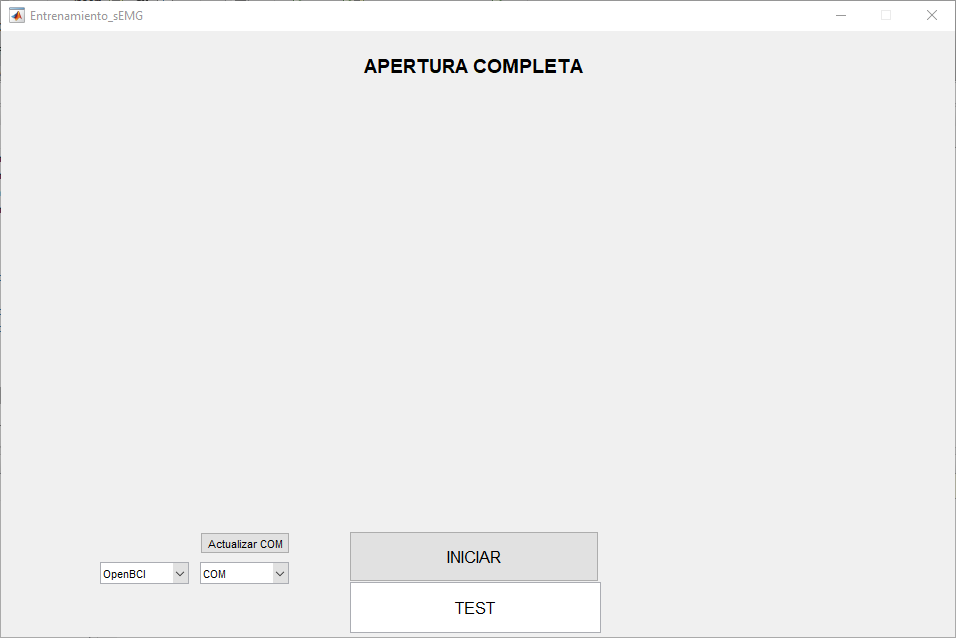
\includegraphics[width=0.7\textwidth]{GUI_Ent.png}
	\caption{GUI utilizada para calibración de amplitud RMS.}
	\label{Figura: GUI_Ent}
\end{figure}

%Posturas manos
\begin{figure}[htbp]
	\centering
	\begin{subfigure}[htbp]{0.4\textwidth}
		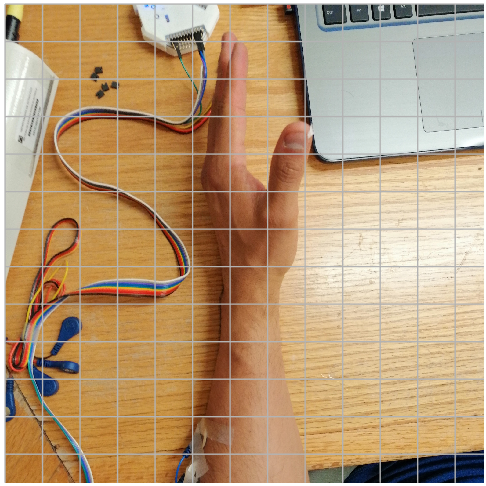
\includegraphics[width=\textwidth]{AI_g.png}
		\caption{}
		\label{Figura: AI}
	\end{subfigure}
%	\hfill
	\begin{subfigure}[htbp]{0.4\textwidth}
		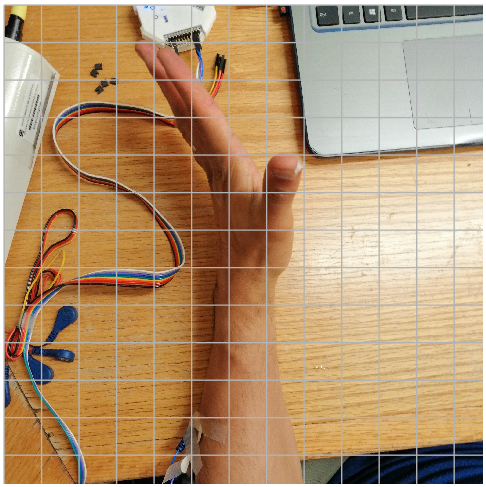
\includegraphics[width=\textwidth]{AC_g.png}
		\caption{}
		\label{Figura: AC}
	\end{subfigure}
%	\hfill
	\newline
	\begin{subfigure}[htbp]{0.4\textwidth}
		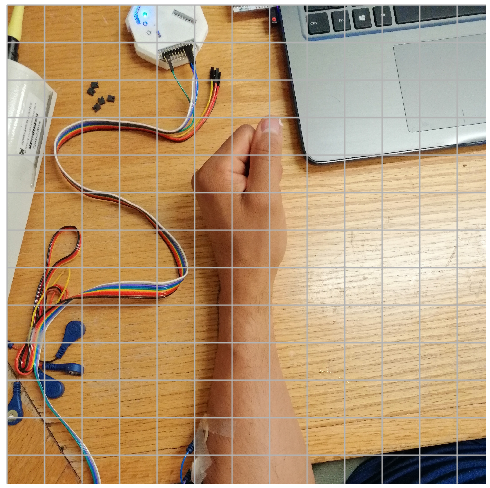
\includegraphics[width=\textwidth]{CI_g.png}
		\caption{}
		\label{Figura: CI}
	\end{subfigure}
%	\hfill
	\begin{subfigure}[htbp]{0.4\textwidth}
		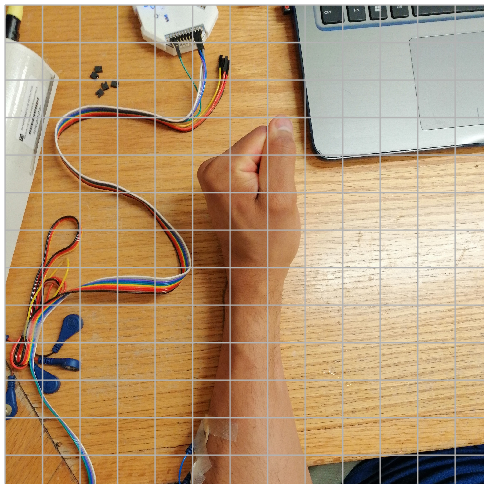
\includegraphics[width=\textwidth]{CC_g.png}
		\caption{}
		\label{Figura: CC}
	\end{subfigure}
%	\hfill
	\newline
	\begin{subfigure}[htbp]{0.4\textwidth}
		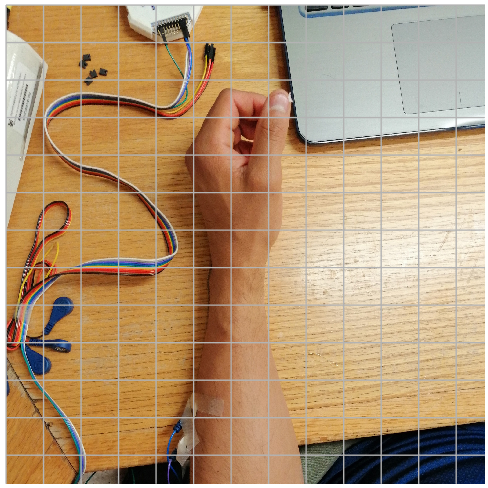
\includegraphics[width=\textwidth]{DD_g.png}
		\caption{}
		\label{Figura: DD}
	\end{subfigure}
	\caption[Posturas de mano para calibración de umbrales RMS]{Posturas de mano para calibración de umbrales RMS de los 5 movimientos. Se agregó una cuadrícula a la imagen para poder observar las diferencias entre las posturas. (a) Apertura de mano incompleta (AI). (b) Apertura de mano completa (AC). (c) Pinza gruesa incompleta (CI). (d) Pinza gruesa completa (CC). (e) Descanso (DD).}
	\label{Figura: Posturas}
\end{figure}

\newpage
\subsection{Validación fuera de línea}
El propósito de esta prueba consiste en obtener un indicador que proporcione información sobre el desempeño del sistema, al configurarlo con los parámetros obtenidos en la calibración, en su función de clasificación de movimientos.

Para obtener dicho indicador se diseñó un script en MATLAB \textregistered \; el cual lleva a cabo el siguiente procedimiento:

\begin{enumerate}
	\item Lectura de registro crudo de sEMG obtenido en etapa de calibración.
	\item Aplicar etapa de procesamiento (filtrado (descrito en la sección \ref{Sec: Procesamiento}), cálculo de RMS y suavizado) a cada ventana de 100 ms de registro de sEMG.
	\item Aplicar algoritmo de control diseñado (FSM y control proporcional) a cada ventana de 100 ms de registro de sEMG.
	\item Clasificar cada ventana de sEMG y generar una matriz de confusión (Cuadro \ref{Cuadro:PorcentajesObtencion}).
	\item Calcular el valor de exactitud global de clasificación para los 3 movimientos (Ecuación \ref{Ecu: Exactitud}).
\end{enumerate}

Una vez obtenido el porcentaje de aciertos y errores, se toma la decisión de aceptar o rechazar los parámetros obtenidos de la calibración. En caso de obtener un porcentaje mayor o igual al 80\% se aceptan los parámetros y se procede a configurar el sistema sEMG-FES diseñado en Simulink \textregistered \; con dichos parámetros. En caso contrario, se revisa la posibilidad de errores en la colocación de electrodos para registro de sEMG y se repite el proceso de calibración.

Cabe mencionar que los registros de calibración se conforman de dos repeticiones de la siguiente secuencia de movimientos:

\begin{enumerate}
	\item Descanso (DD): 9 segundos
	\item Pinza gruesa incompleta (CI): 3 segundos
	\item Pinza gruesa completa (CC): 6 segundos
	\item Pinza gruesa incompleta (CI): 3 segundos
	\item Descanso (DD): 9 segundos
	\item Apertura de mano incompleta (AI): 3 segundos
	\item Apertura de mano completa (AC): 6 segundos
	\item Apertura de mano incompleta (AI): 3 segundos
\end{enumerate}

%Cuadro porcentajes aciertos y errores 
\begin{table}[htbp]
	\centering
	\begin{tabular}{|l|c|c|c|}
	\hline
	\textbf{} & \multicolumn{3}{|c|}{Movimiento real}\\
	\textbf{Movimiento} & \textbf{Descanso} & \textbf{Pinza} & \textbf{Apertura}\\
	\textbf{predicho} & \textbf{} & \textbf{gruesa} & \textbf{de mano}\\ \hline \hline
	\textbf{Descanso} & \textbf{TD} & \textbf{FDC} & \textbf{FDA}\\ \hline
	\textbf{Pinza gruesa} & \textbf{FCD} & \textbf{TC} & \textbf{FCA}\\ \hline
	\textbf{Apertura de mano} & \textbf{FAD} & \textbf{FAC} & \textbf{TA}\\ \hline
	\end{tabular}
	\caption{Matriz de confusión para prueba fuera de línea.}
	\label{Cuadro:PorcentajesObtencion}
\end{table}

\begin{equation}
	Exactitud = \frac{T}{T+FDC+FDA+FCD+FCA+FAD+FAC}\times100\%
	\label{Ecu: Exactitud}
\end{equation}

Donde $T = TD+TC+TA$. $TD$, $TC$ y $TA$ corresponden a los movimientos \emph{descanso}, \emph{pinza gruesa} y \emph{apertura de mano}, respectivamente, clasificados de forma correcta. $FDC$ corresponde al movimiento \emph{descanso} clasificado como \emph{pinza gruesa}. $FDA$ corresponde al movimiento \emph{descanso} clasificado como \emph{apertura de mano}. $FCD$ corresponde al movimiento \emph{pinza gruesa} clasificado como \emph{descanso}. $FCA$ corresponde al movimiento \emph{pinza gruesa} clasificado como \emph{apertura de mano}. $FAD$ corresponde al movimiento \emph{apertura de mano} clasificado como \emph{descanso}. $FAC$ corresponde al movimiento \emph{apertura de mano} clasificado como \emph{pinza gruesa}.

\subsection{Validación en línea (control por biofeedback)}
Una vez que el sistema se ha validado fuera de línea, se procede a realizar una prueba para corroborar su funcionamiento en línea. Para llevar a cabo esto se utiliza el sistema sEMG-FES en línea implementado en Simulink\textregistered \; (Figura \ref{Figura: SisComp}) configurándolo de la siguiente manera:

\begin{enumerate}
	\item Se configura el bloque \emph{Control} con los valores de los parámetros obtenidos en la calibración.
	\item Se conecta el switch \emph{Habilitar estimulación} a \emph{Ceros} para evitar la salida de estimulación eléctrica real, pues en esta validación no se usa.
	\item Se configura el tiempo de término de la simulación con un valor de 60 s.
\end{enumerate}

%Sistema completo
\begin{figure}[htbp]
	\centering
	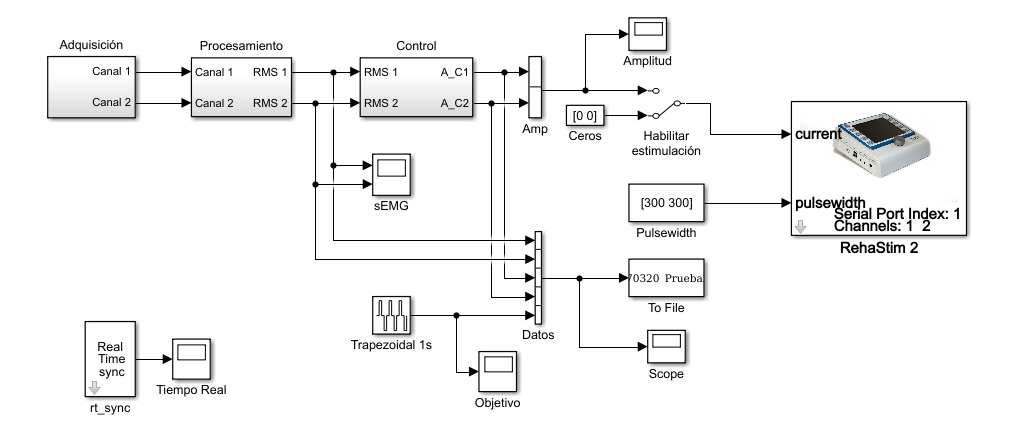
\includegraphics[width=\textwidth]{SistemaCompleto.png}
	\caption{Diagrama de bloques del sistema sEMG-FES en línea implementado en Simulink\textregistered.}
	\label{Figura: SisComp}
\end{figure}

\newpage
Posteriormente, se le indica al sujeto la forma en la que se llevará a cabo la prueba y cómo deberá realizarla. Para esto, al sujeto se le mostrará en una ventana una señal trapezoidal con ciclos negativos y ciclos positivos (Figura \ref{Figura: Trapezoidal}), el sujeto deberá realizar el seguimiento de dicha trapezoidal considerando que el ciclo positivo indica apertura de mano completa, mientras que el ciclo negativo indica pinza gruesa completa y que una línea en cero indica la mano en posición de descanso. El sujeto deberá realizar una transición suave y continua entre los movimientos indicados buscando seguir visualmente las pendientes de la trapezoidal. Una vez dadas las indicaciones se inicia la prueba, y a la par el experimentador deberá observar en otra ventana la salida del bloque de control, donde se observará si la activación de canales de estimulación eléctrica corresponden a los movimientos que realiza el sujeto. La respuesta esperada del sistema consiste en que, la detección de un movimiento de pinza gruesa activa el canal 1 de estimulación, y la detección del movimientos de apertura de mano activa el canal 2 de estimulación.

\vfill
%Trapezoidal
\begin{figure}[htbp]
	\centering
	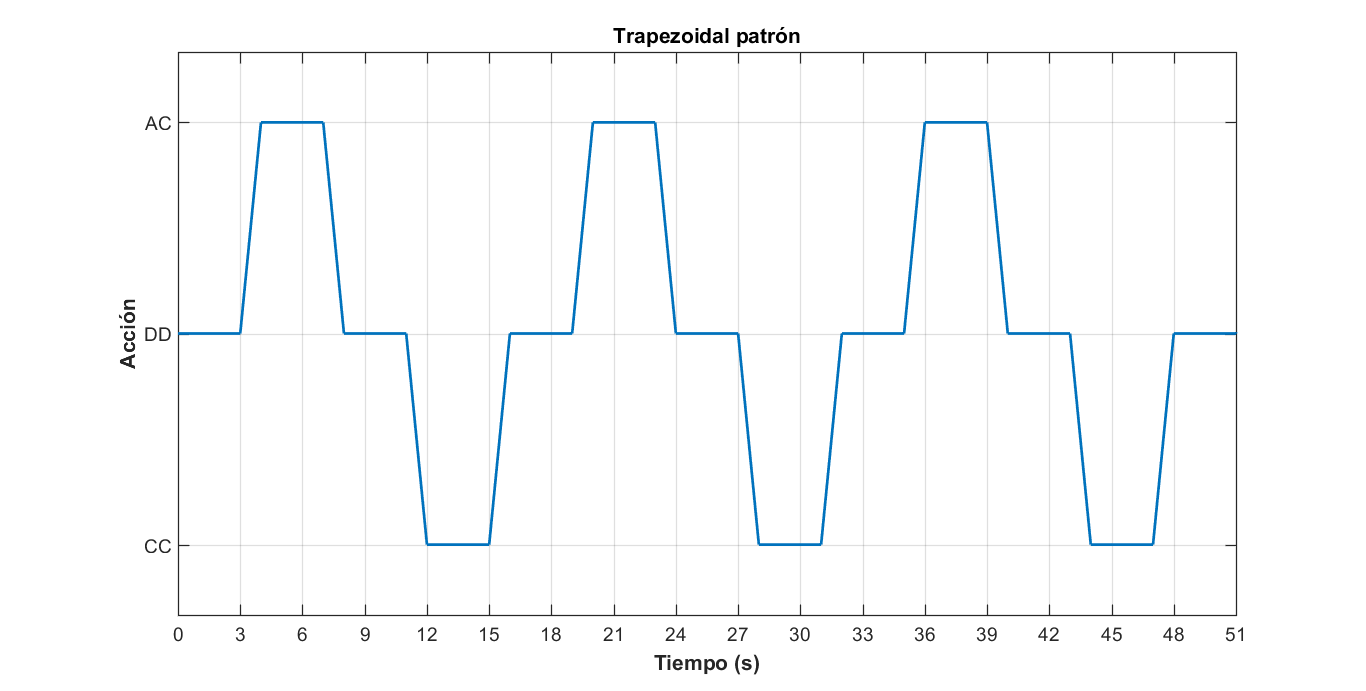
\includegraphics[width=\textwidth]{Trapezoidal.png}
	\caption[Segmento de señal trapezoidal patrón]{Segmento de señal trapezoidal utilizada como guía visual para el sujeto en la prueba en línea. El ciclo positivo indica al sujeto que realice un movimiento de apertura de mano (AC), el ciclo negativo indica al sujeto que realice un movimiento de pinza gruesa (CC), mientras que el valor en cero indica que realice un descanso (DD). El inicio de las mesetas inferior y superior de la señal trapezoidal indican al sujeto el momento en el que debería llegar al rango completo del movimiento correspondiente, y la duración de estas mesetas indican el tiempo que debe mantener el movimiento con rango de movimiento completo (contracción isométrica).}
	\label{Figura: Trapezoidal}
\end{figure}
\vfill

\newpage
\subsection{Validación en línea con FES}\label{Sec: TareaObj}
En esta prueba final se utilizan los mismos parámetros e indicaciones que en la prueba de validación en línea, sin embargo, para esta prueba se aplica estimulación eléctrica al brazo afectado del sujeto, por lo que el switch \emph{Habilitar estimulación} se encuentra conectada la salida del bloque \emph{Control}, y además, el tiempo de término de la simulación se configura a 180 s.

En esta prueba se mide el tiempo de retardo que existe entre el inicio del movimiento en la mano ``sana'' (generado de manera voluntaria) y el inicio del movimiento en la mano afectada (generado por FES). Para poder realizar esto se almacenan todos los datos de las señales involucradas en el sistema (registros de sEMG, patrones de estimulación eléctrica y señal trapezoidal patrón), y posterior a la finalización de la prueba se realiza un análisis en MATLAB\textregistered \; donde se determina el tiempo de retardo existente entre el inicio de la señal trapezoidal (indicación al sujeto) y el inicio de la estimulación en el canal de estimulación del movimiento correspondiente, y se obtiene el promedio del retardo de todas las repeticiones realizadas para obtener un retardo global de la sesión.

\subsection{Tarea funcional asíncrona}\label{Sec: TareaFunAsin}
Se diseñó una prueba de tiempo libre donde pudiera demostrarse la utilidad del sistema diseñado para realizar alguna tarea funcional útil para el sujeto. Para esta prueba se configuró el sistema sEMG-FES de la misma forma en la cual se configuró dicho sistema para la realización de la validación en línea con FES, pero cambiando el tiempo de término de la simulación en Simulink \textregistered\; al valor \emph{inf}. Para esta prueba los antebrazos y manos del sujeto descansan sobre una mesa, en la cual se colocan dos objetos cilíndricos a unos centímetros de sus manos (un objeto en cada mano). Una vez configurado el sistema sEMG-FES y colocado el sujeto en la posición adecuada, se procede a llevar a cabo la tarea funcional asíncrona. Esta tarea se explica en el Cuadro \ref{Cuadro:TareaFunAsin}, donde se describen los diferentes movimientos a realizar por el sujeto, el comportamiento esperado en los diferentes canales de sEMG, el canal FES que debería activar dicho movimiento, el movimiento generado por FES que se espera, y la correspondencia de dicho movimiento con su representación gráfica en la Figura \ref{Figura: TareaFuncional_P}.

Cabe mencionar que desde los incisos (c) al (e) del Cuadro \ref{Cuadro:TareaFunAsin} , el sujeto debe sostener (contracción isométrica) el movimiento voluntario de pinza gruesa en la mano izquierda, y se espera esto genere la estimulación eléctrica necesaria para sostener el objeto con la mano derecha, sin que el sujeto realice algún esfuerzo voluntario en dicha mano, imitando la condición de hemiplejia de un sujeto con ACV.

%Cuadro descriptivo de tarea funcional
\begin{table}[htbp]
	\centering
	\begin{tabular}{|p{5cm}|p{1.4cm}|p{1.4cm}|p{3.5cm}|p{1.5cm}|}
	\hline
	\textbf{Movimiento voluntario} & \textbf{Canal sEMG activo} & \textbf{Canal FES activo} & \textbf{Movimiento FES} & \textbf{Figura}\\ \hline \hline
	Adducción del hombro en ambos brazos para acercar mano a objeto cilíndrico cercano. & Nulo. & Nulo. & Ninguno. & Figura \ref{Figura: TareaFuncional_P}(a)\\ \hline
	Extensión de dedos con mano ``sana'' (izquierda). En ambos brazos se deberá acercar la palma abierta al objeto correspondiente. & 2 & 2 & Apertura de mano ``afectada'' (derecha). & Figura \ref{Figura: TareaFuncional_P}(b)\\ \hline
	Flexión de dedos con mano "sana" (izquierda) para lograr tomar el objeto. & 1 & 1 & Pinza gruesa en mano ``afectada'' (derecha) para tomar objeto. & Figura \ref{Figura: TareaFuncional_P}(c)\\ \hline
	Abducción y extensión de ambos hombros para levantar objetos 10 cm de la mesa y trasladarlos lateralmente 10 cm de su posición original. & 1 & 1 & Pinza gruesa en mano ``afectada'' (derecha) & Figura \ref{Figura: TareaFuncional_P}(d)\\ \hline
	Flexión de ambos hombros para bajar objetos a la altura de la mesa. & 1 & 1 & Pinza gruesa en mano ``afectada'' (derecha) & Figura \ref{Figura: TareaFuncional_P}(e)\\ \hline
	Extensión de dedos con mano ``sana'' (izquierda) para soltar objeto sobre la mesa. & 2 & 2 & Apertura de mano ``afectada'' (derecha) para soltar objeto sobre la mesa. & Figura \ref{Figura: TareaFuncional_P}(f)\\ \hline
	\end{tabular}
	\caption{Descripción detallada de tarea funcional asíncrona.}
	\label{Cuadro:TareaFunAsin}
\end{table}

%Figura tarea funcional (manitas)
\begin{figure}[htbp]
	\centering
	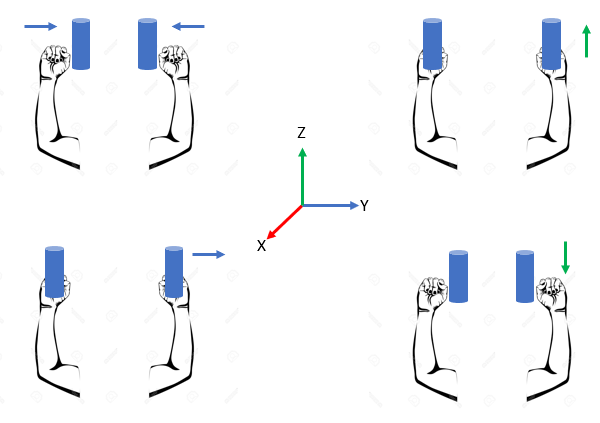
\includegraphics[width=\textwidth]{TareaFuncional.png}
	\caption[Esquema de tarea funcional con tiempo libre.]{Esquema de tarea funcional con tiempo libre. Las flechas indican la dirección de cada movimiento de las manos o brazos. Tomando como referencia la posición corporal del sujeto para esta tarea, las flechas azules indican movimientos en el eje Y (plano corporal frontal), las flechas rojas indican movimientos en el eje X (plano corporal transversal), y las flechas verdes indican movimientos en el eje Z (plano corporal sagital).Cada inciso corresponde a un movimiento descrito en el Cuadro \ref{Cuadro:TareaFunAsin}.}
	\label{Figura: TareaFuncional_P}
\end{figure}


\chapter{Resultados}
%%RESULTADOS

\section{Evaluación de bloque de adquisición y decodificación}
Tras realizar la evaluación del subsistema de adquisición descrito en la sección \ref{Sec: Adquisicion} utilizando el procedimiento detallado en la sección \ref{Sec: EvalAdquisicion}, se obtuvo un valor de correlación promedio de 0.9615 $\pm$ 0.0604, el cual se obtuvo de un total de 27 registros realizados (3 repeticiones de cada una de las señales que conforman el banco de señales para evaluación de la adquisición). En la Figura \ref{Figura: ValProCum} se puede observar una comparación entre la señal patrón de 5 Hz y la señal adquirida con el subsistema diseñado en Simulink\textregistered. El Cuadro \ref{Cuadro:ValoresCorre} muestra el valor de correlación promedio obtenido para cada señal y la correlación total.

%Cuadro valores correlación
\begin{table}[htbp]
	\centering
	\begin{tabular}{|l|c|}
	\hline
	\textbf{} & \textbf{Correlación}\\ 
	\textbf{Señal} & \textbf{promedio}\\ \hline	\hline
	1 Hz & 0.9889\\ \hline
	5 Hz & 0.9428\\ \hline
	10 Hz & 0.9948\\ \hline
	20 Hz & 0.9933\\ \hline
	50 Hz & 0.9804\\ \hline
	100 Hz & 0.9334\\ \hline
	Atenuación lineal & 0.9466\\ \hline
	Atenuación exponencial & 0.8849\\ \hline
	Simulación contracción muscular & 0.9886\\ \hline
	\textbf{Correlación promedio total} & 0.9615\\ \hline
	\end{tabular}
	\caption{Valores de correlación promedio por señal y correlación promedio total.}
	\label{Cuadro:ValoresCorre}
\end{table}

%Senoidal obtenida tras para evaluación
\begin{figure}[htbp]
	\centering
	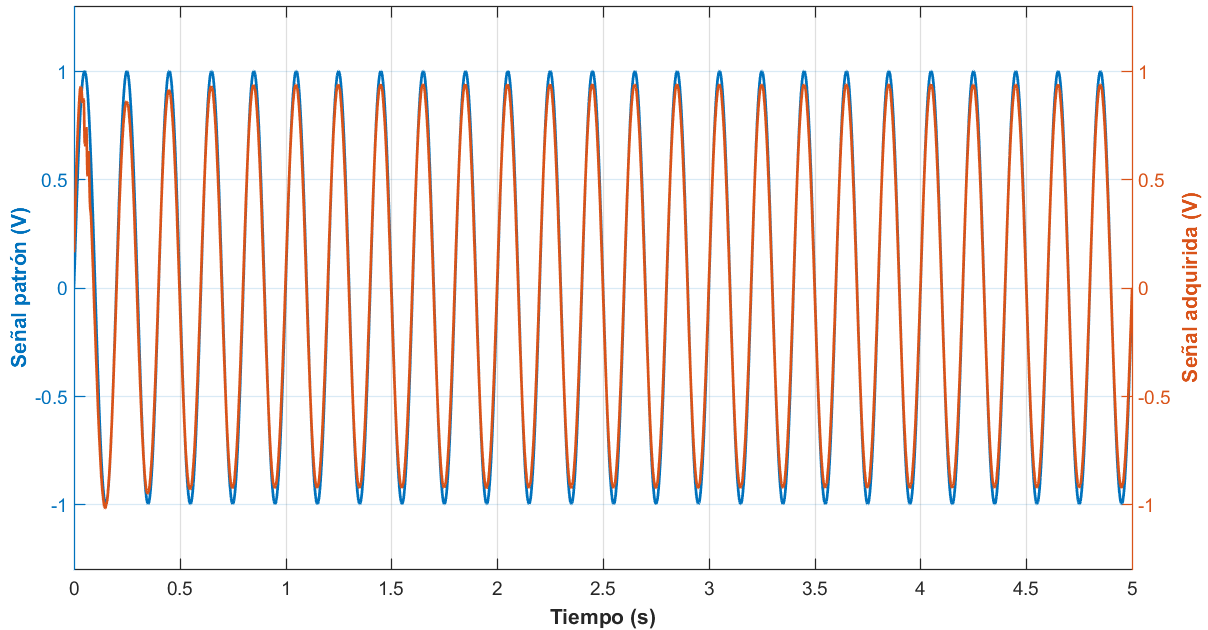
\includegraphics[width=\textwidth]{ValProCum.png}
	\caption[Comparación entre señales para evaluación de adquisición.]{Comparación entre señales para evaluación de adquisición. Señal patrón generada en MATLAB\textregistered \; (azul). Señal adquirida mediante el subsistema de adquisición diseñado en Simulink\textregistered \; (Rojo).}
	\label{Figura: ValProCum}
\end{figure}


\newpage
\section{Procesamiento de sEMG}
El esquema de filtrado utilizado (filtro pasa altas, filtro pasa bajas y filtro rechaza banda), al igual que el procesamiento para obtención del RMS suavizado, se pusieron a prueba fuera de línea con registros de sEMG de 10 voluntarios sanos (6 hombres y 4 mujeres en el rango de 20 a 24 años de edad).

La Figura \ref{Figura: Filtrado} muestra una comparación entre los canales de sEMG adquiridos para las pruebas de procesamiento y el resultado del filtrado fuera de línea. En la Figura \ref{Figura: RMS} se muestra un ejemplo del resultado del procesamiento para obtención de la envolvente RMS suavizada.

\begin{figure}[htbp]
	\centering
	\begin{subfigure}[htbp]{0.45\textwidth}
		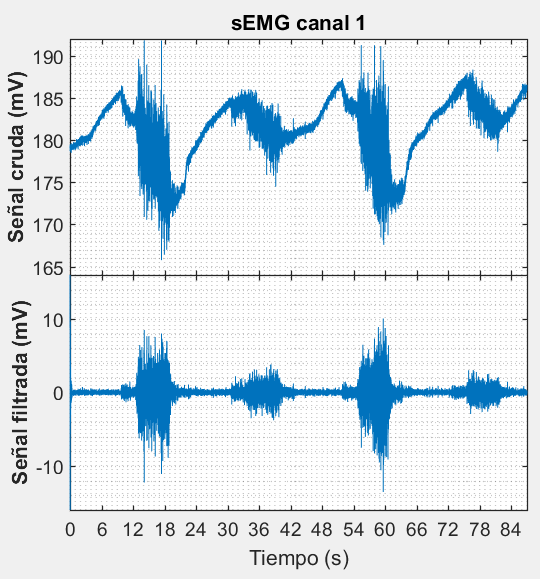
\includegraphics[width=\textwidth]{Filtrado_a.png}
		\caption{}
		\label{Figura: Filtrado_a}
	\end{subfigure}
	\hfill
	\begin{subfigure}[htbp]{0.45\textwidth}
		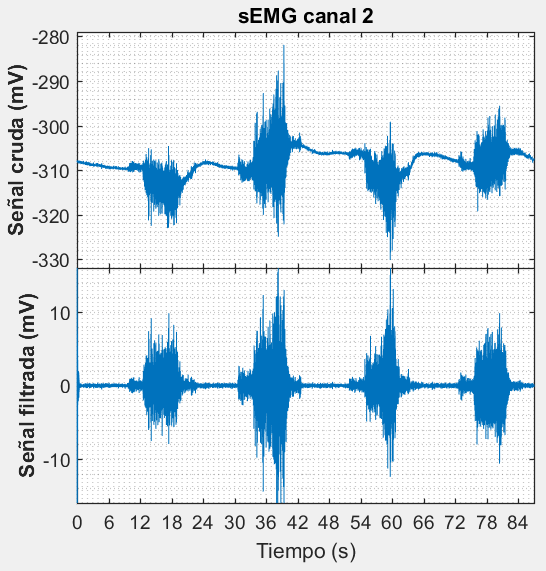
\includegraphics[width=\textwidth]{Filtrado_b.png}
		\caption{}
		\label{Figura: Filtrado_b}
	\end{subfigure}	
	\caption[Ejemplo representativo del funcionamiento del esquema de filtrado diseñado]{Ejemplo representativo del funcionamiento del esquema de filtrado diseñado.(a)Arriba, registro de sEMG del canal 1 sin filtrar.(a)Abajo, registro de sEMG del canal 1 después del filtrado.(b)Arriba, registro de sEMG del canal 2 sin filtrar.(b)Abajo, registro de sEMG del canal 2 después del filtrado.}
	\label{Figura: Filtrado}
\end{figure}

\begin{figure}[htbp]
	\centering
	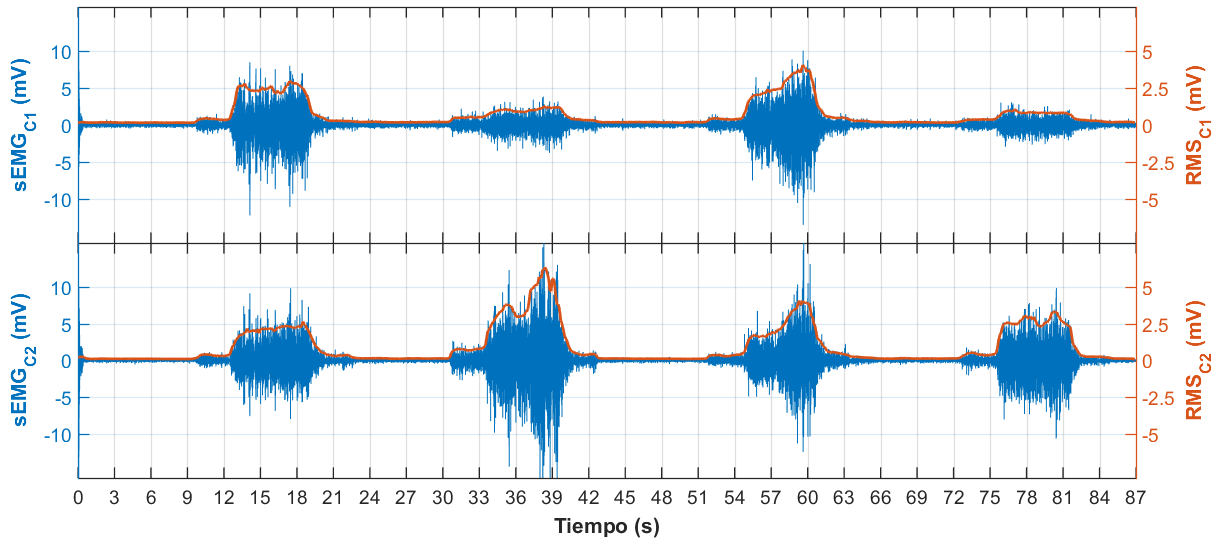
\includegraphics[width=\textwidth]{RMS.png}
	\caption[Ejemplo representativo de la obtención de envolvente de RMS]{Ejemplo representativo de la obtención de envolvente de RMS. En azul, los registros de sEMG después del filtrado. En rojo, las envolventes de RMS. Arriba, señal sEMG y envolvente del canal 1, correspondiente al movimiento de pinza gruesa. Abajo, señal sEMG y envolvente del canal 2, correspondiente al movimiento de apertura de mano.}
	\label{Figura: RMS}
\end{figure}


\newpage
\section{Sistema de control}
El sistema de control sEMG-FES se puso a prueba con un voluntario sano de 22 años de edad, obteniendo los siguientes resultados.

\subsection{Calibración}
Tras realizar el proceso de calibración descrito en la sección \ref{Sec: Calibracion} se obtuvieron los valores mostrados en los Cuadros \ref{Cuadro:UmbralesFES} a \ref{Cuadro:Rectas}.

El Cuadro \ref{Cuadro:UmbralesFES} muestra los valores obtenidos para los umbrales motores y funcionales tras realizar la calibración de parámetros FES descrita en la sección \ref{Sec:CalFES}.

El Cuadro \ref{Cuadro:UmbralesRMS} muestra los valores de umbrales RMS y el valor del umbral detector de movimiento obtenidos tras realizar la calibración de umbrales RMS de sEMG descrita en la sección \ref{Sec:CalRMS}. Cabe señalar que en esta prueba se obtuvo un umbral de activación menor para el movimiento de pinza gruesa en comparación con el umbral de activación para el movimiento de apertura de mano (recordemos que los umbrales de activación son el umbral de pinza gruesa incompleta en el canal 1 y el umbral de apertura de mano incompleta en el canal 2).

El Cuadro \ref{Cuadro:Rectas} muestra los valores de la pendiente y la ordenada al origen correspondientes a las rectas de mapeo proporcional para el canal 1 y el canal 2 de estimulación eléctrica.

%Cuadro umbrales FES
\begin{table}[htbp]
	\centering
	\begin{tabular}{|l|c|c|}
	\hline
	\textbf{} & \textbf{Umbral motor} & \textbf{Umbral funcional}\\
	\textbf{} & \textbf{($U_{Mj}$)} & \textbf{($U_{Fj}$)}\\
	\textbf{Canal} & \textbf{[mA]} & \textbf{[mA]}\\ \hline	\hline
	Canal 1 (Pinza gruesa) & 6 & 14\\ \hline
	Canal 1 (Apertura de mano) & 9 & 13\\ \hline
	\end{tabular}
	\caption{Valores obtenidos para umbrales motores y funcionales de estimulación eléctrica.}
	\label{Cuadro:UmbralesFES}
\end{table}

%Cuadro umbrales sEMG
\begin{table}[htbp]
	\centering
	\begin{tabular}{|l|c|c|}
	\hline
	\textbf{} & \multicolumn{2}{|c|}{Umbral RMS}\\
	\textbf{} & \textbf{Canal 1} & \textbf{Canal 2}\\
	\textbf{} & \textbf{$j=1$} & \textbf{$j=2$}\\
	\textbf{Movimiento} & \textbf{[mV]} & \textbf{[mV]}\\ \hline \hline
	Apertura de mano completa ($M_{1j}$) & 0.8708 & 3.0000\\ \hline
	Apertura de mano incompleta	($M_{2j}$) & 0.4657 & 0.9115\\ \hline
	Descanso ($M_{3j}$) & 0.1981 & 0.1536\\ \hline
	Pinza gruesa incompleta ($M_4j$) & 0.7918 & 0.8134\\ \hline
	Pinza gruesa completa ($M_5j$) & 2.2491 & 1.9610\\ \hline	
	Umbral detector de movimiento ($UDM$) & \multicolumn{2}{|c|}{0.4458}\\ \hline
	\end{tabular}
	\caption{Valores obtenidos para umbrales RMS de sEMG.}
	\label{Cuadro:UmbralesRMS}
\end{table}

%Cuadro parámetros de rectas
\begin{table}[htbp]
	\centering
	\begin{tabular}{|l|c|c|}
	\hline
	\textbf{} & \textbf{Pendiente} & \textbf{Ordenada al origen}\\ 
	\textbf{} & \textbf{($m_{j}$)} & \textbf{($b_{j}$)}\\
	\textbf{Canal} & \textbf{[mA/mV]} & \textbf{[mA]}\\\hline \hline
	Canal 1 (Pinza gruesa) & 5.4894 & 1.6536\\ \hline
	Canal 2 (Apertura de mano) & 1.9153 & 7.2542\\ \hline
	\end{tabular}
	\caption{Parámetros de recta obtenidos para realizar mapeo sEMG-FES.}
	\label{Cuadro:Rectas}
\end{table}


\newpage
\subsection{Validación fuera de línea}
El algoritmo de clasificación de movimientos obtuvo una exactitud del 81.7241\%, valor derivado de la matriz de confusión mostrada en el Cuadro \ref{Cuadro:PorcentajesValores}. La Figura \ref{Figura: MapOff} muestra el resultado de la prueba para la validación fuera de línea, donde se pueden observar los siguientes resultados de clasificación:

\begin{itemize}
	\item Durante los episodios del movimiento de cierre de mano (9-21 y 51-63 s):
	
	\begin{itemize}
		\item Se puede observar una clasificación correcta cuando la señal \emph{Acción} toma como valores a \emph{CI} y \emph{CC} y la señal \emph{Amplitud FES$_{C1}$} toma valores distintos de cero mientras que la señal \emph{Amplitud FES$_{C2}$} toma valor de cero.
		\item Dentro de los episodios de este movimiento se pueden observar errores de clasificación en los segundos 18-21 y alrededor de los 59 segundos, donde se observa que la señal \emph{Amplitud FES$_{C2}$} toma valores distintos de cero.
	\end{itemize}
	
	\item Durante los episodios del movimiento de apertura de mano (30-42 y 72-84 s):
	
	\begin{itemize}
		\item Se puede observar una clasificación correcta cuando la señal \emph{Acción} toma como valores a \emph{AI} y \emph{AC} y la señal \emph{Amplitud FES$_{C2}$} toma valores distintos de cero mientras que la señal \emph{Amplitud FES$_{C1}$} toma valor de cero.
		\item Dentro de los episodios de este movimiento se pueden observar errores de clasificación en los segundos 30-33, 40-42 y 72-75, donde se observa que la señal \emph{Amplitud FES$_{C1}$} toma valores distintos de cero.
	\end{itemize}
		
	\item Durante los episodios de descanso (0-9, 21-30, 42-51, 63-72 y 84-87 s):
	\begin{itemize}
		\item Se puede observar una clasificación correcta cuando la señal \emph{Acción} toma como valor a \emph{DD} y las señales \emph{Amplitud FES$_{C1}$} y \emph{Amplitud FES$_{C2}$} toman valor de cero.
		\item Dentro de los episodios de este movimiento se pueden observar errores alrededor de los segundos 42 y 63, donde la señal \emph{Amplitud FES$_{C1}$} se activa brevemente cuando no tendría que haberse activado.
	\end{itemize}
\end{itemize}

%Cuadro porcentajes aciertos y errores 
\begin{table}[htbp]
	\centering
\begin{tabular}{|l|c|c|c|}
	\hline
	\textbf{} & \multicolumn{3}{|c|}{Movimiento real}\\
	\textbf{Movimiento} & \textbf{Descanso} & \textbf{Pinza} & \textbf{Apertura}\\
	\textbf{predicho} & \textbf{} & \textbf{gruesa} & \textbf{de mano}\\ \hline \hline
	\textbf{Descanso} & \textbf{381} & \textbf{9} & \textbf{0}\\ \hline
	\textbf{Pinza gruesa} & \textbf{41} & \textbf{192} & \textbf{7}\\ \hline
	\textbf{Apertura de mano} & \textbf{32} & \textbf{70} & \textbf{138}\\ \hline
	\end{tabular}
	\caption{Matriz de confusión obtenida tras validación fuera de línea.}
	\label{Cuadro:PorcentajesValores}
\end{table}

%Figura validación fuera de línea
\begin{figure}[htbp]
	\centering
	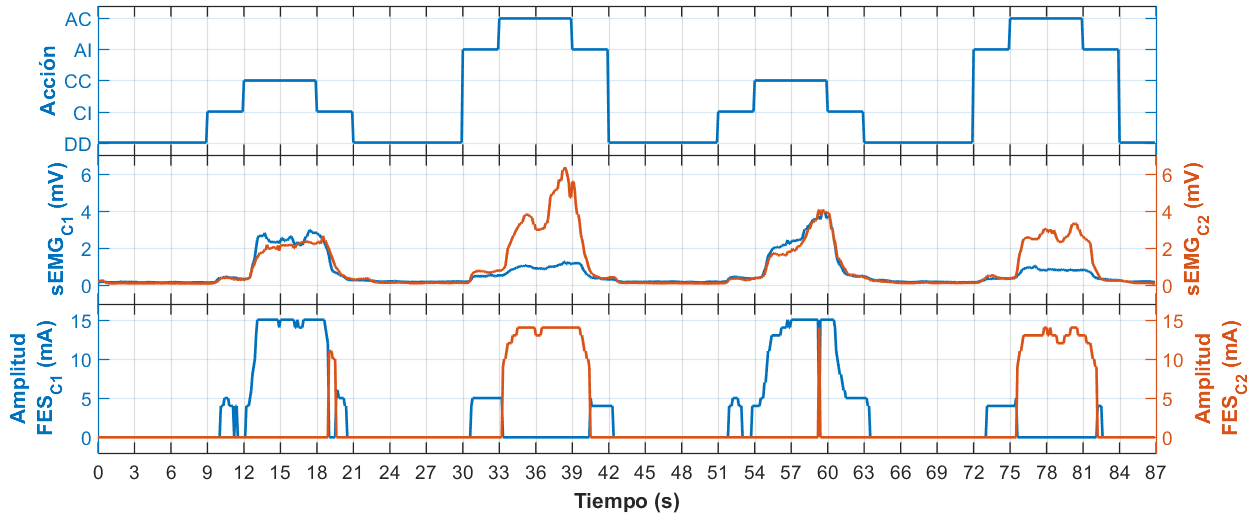
\includegraphics[width=\textwidth]{MapOff.png}
	\caption[Secuencia temporal de una prueba exitosa de validación fuera de línea]{Secuencia temporal de una prueba exitosa de validación fura de línea del sistema de control sEMG-FES. Arriba: Marcadores de acción solicitada al sujeto (descanso (DD), pinza gruesa incompleta (CI), pinza gruesa completa (CC), apertura de mano incompleta (AL), apertura de mano completa (AC)). Centro: Envolventes de sEMG (Azul: canal 1. Rojo: canal 2). Abajo: Amplitudes de estimulación eléctrica (salida del sistema de control) (Azul: canal 1. Rojo: canal 2). }
	\label{Figura: MapOff}
\end{figure}


\newpage
\subsection{Validación en línea (control por biofeedback)}
Respecto a la prueba de validación en línea, en esta demostró una respuesta del sistema de acuerdo a lo esperado. La Figura \ref{Figura: MapOn} presenta un segmento de las señales obtenidas tras la realización de la prueba en línea.

%Figura prueba en línea (sin estimulación)
\begin{figure}[htbp]
	\centering
	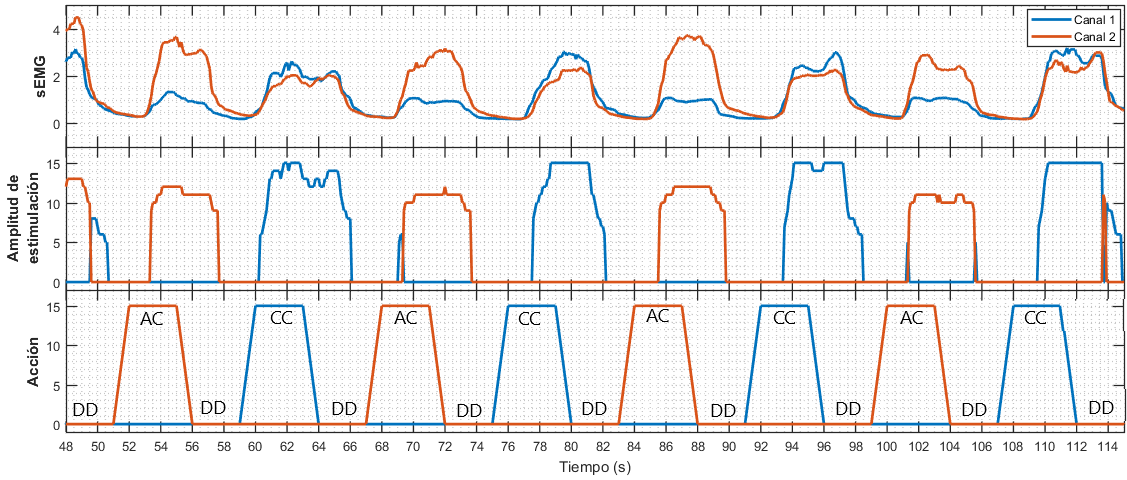
\includegraphics[width=\textwidth]{MapOn.png}
	\caption[Secuencia temporal de una prueba exitosa de validación en línea]{Secuencia temporal de una prueba exitosa de validación en línea del sistema de control sEMG-FES.  Arriba: Señal trapezoidal patrón indicadora del movimiento objetivo (descanso (DD), pinza gruesa (CC), apertura de mano completa (AC)). Centro: Envolventes de sEMG (Azul: canal 1. Rojo: canal 2). Abajo: Amplitudes de estimulación eléctrica (salida del sistema de control) (Azul: canal 1. Rojo: canal 2).}
	\label{Figura: MapOn}
\end{figure}


\subsection{Validación en línea con FES}
En relación a la validación en línea con FES, el sistema logró llevar a cabo la modulación de la estimulación eléctrica de forma satisfactoria, obteniendo un retardo promedio del sistema con valor de de 2.3 $\pm$ 0.3553 s, medido de la forma descrita en la sección \ref{Sec: TareaObj}. La Figura \ref{Figura: Retardo} muestra un acercamiento a las señales obtenidas al termino de la prueba de la validación en línea con FES, donde se aprecia el retardo entre la señal patrón y la señal de amplitud de estimulación eléctrica.

\newpage
%Figura medición de retardo
\begin{figure}[htbp]
	\centering
	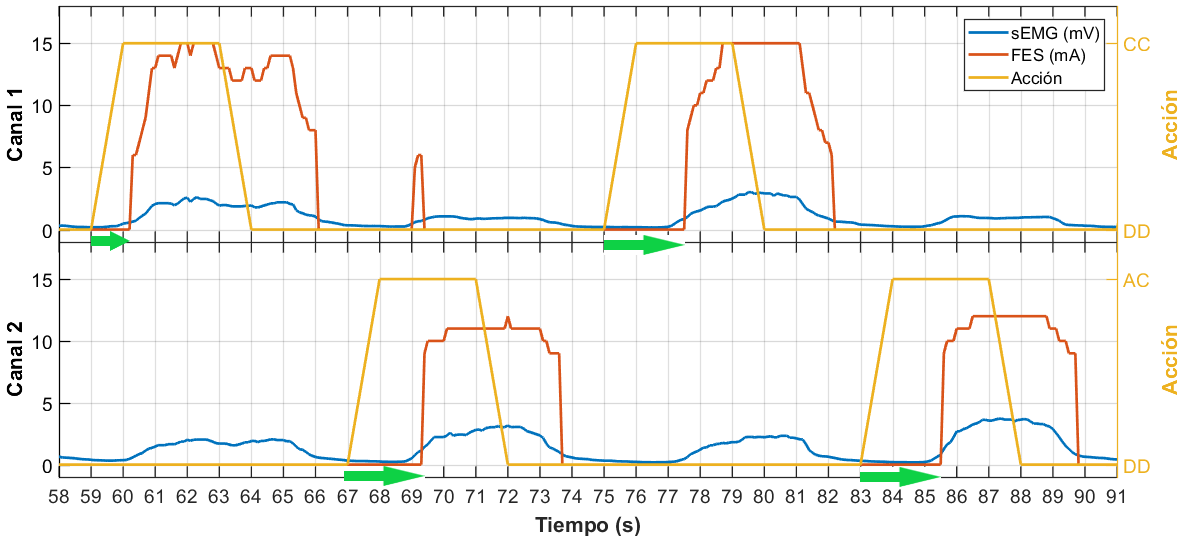
\includegraphics[width=\textwidth]{Retardo_Flechas_2.png}
	\caption[Secuencia temporal de una prueba exitosa de la validación en línea con FES]{Secuencia temporal de una prueba exitosa de la validación en línea con FES. Se muestran las diferentes señales asociadas a cada movimiento sobre la misma base de tiempo para visualizar el retardo existente entre la señal trapezoidal patrón y la señal de amplitud de estimulación eléctrica. Arriba: Señales para movimiento pinza gruesa completa (CC). Abajo: Señales para movimiento apertura de mano completa (AC). En amarillo se muestra la señal trapezoidal patrón del movimiento objetivo. En azul se muestra la envolvente de sEMG. En rojo se muestra la amplitud de estimulación eléctrica (salida del sistema control). Se agregaron flechas color verde a las gráficas para resaltar el retardo existente entre la señal trapezoidal y la amplitud FES. La escala vertical mostrada a la izquierda es la misma para las señales sEMG y FES, sólo se aplica el correspondiente cambio de unidades.}
	\label{Figura: Retardo}
\end{figure}


\subsection{Tarea funcional asíncrona}
Respecto a la tarea funcional asíncrona, esta logró ser realizada por el sujeto de prueba, logrando realizar las 6 acciones de la que consta dicha tarea. La Figura \ref{Figura: TareaFuncional} muestra las diferentes fases de movimiento durante la ejecución de la tarea funcional asíncrona por parte del sujeto, mientras que la Figura \ref{Figura: TareaFuncional_Senales} muestra las señales (sEMG y FES) correspondiente a cada fase. Se puede apreciar que los movimientos corresponden a los descritos en la sección \ref{Sec: TareaFunAsin}.

%Figura levantar objetos
\begin{figure}[htbp]
	\centering
	\begin{subfigure}[htbp]{0.45\textwidth}
		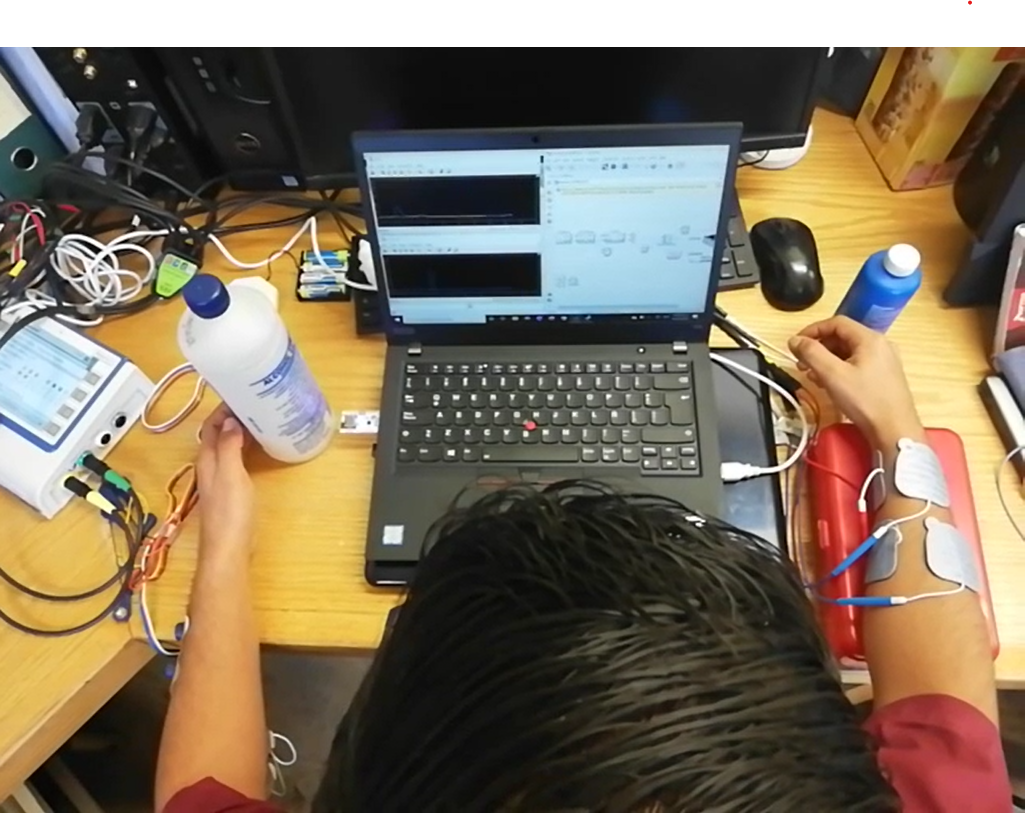
\includegraphics[width=\textwidth]{Funcional_a.png}
		\caption{}
		\label{Figura: Fun_A}
	\end{subfigure}
	\begin{subfigure}[htbp]{0.45\textwidth}
		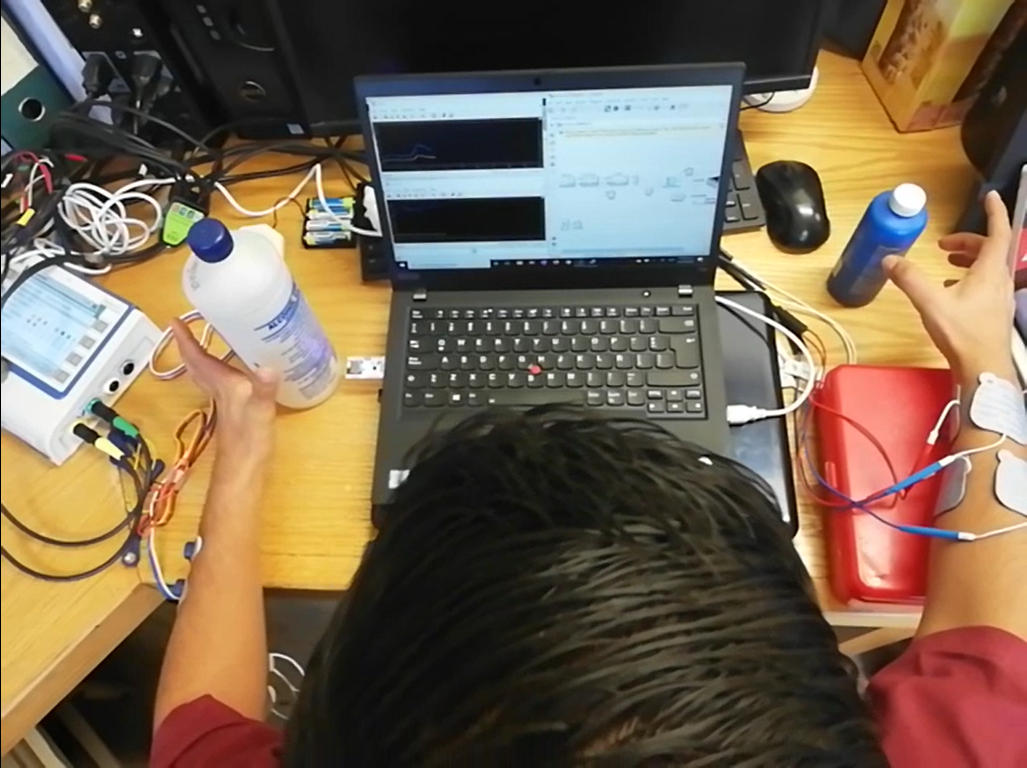
\includegraphics[width=\textwidth]{Funcional_b.png}
		\caption{}
		\label{Figura: Fun_B}
	\end{subfigure}
	\newline
	\begin{subfigure}[htbp]{0.45\textwidth}
		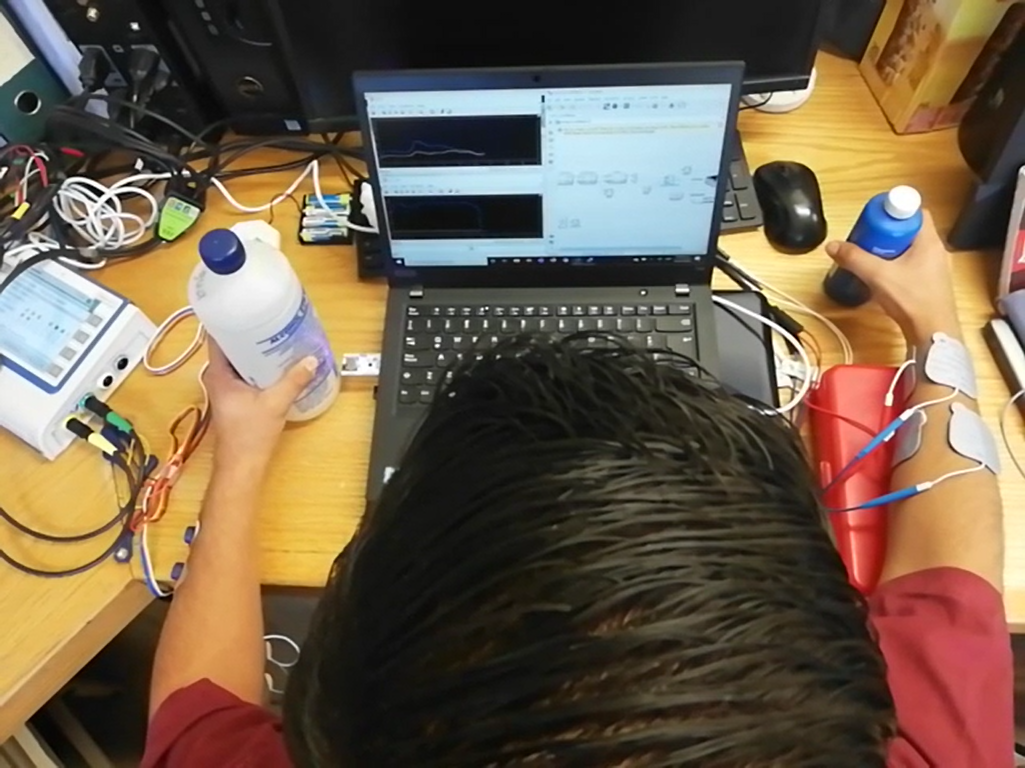
\includegraphics[width=\textwidth]{Funcional_c.png}
		\caption{}
		\label{Figura: Fun_C}
	\end{subfigure}
	\begin{subfigure}[htbp]{0.45\textwidth}
		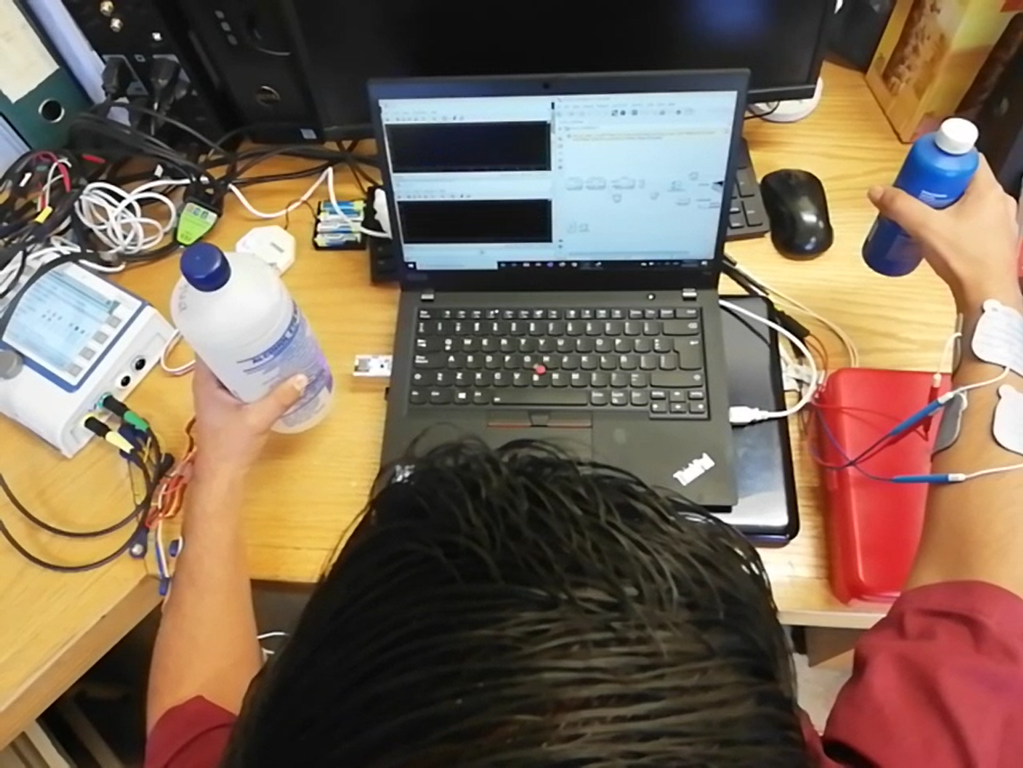
\includegraphics[width=\textwidth]{Funcional_d.png}
		\caption{}
		\label{Figura: Fun_D}
	\end{subfigure}
	\newline
	\begin{subfigure}[htbp]{0.45\textwidth}
		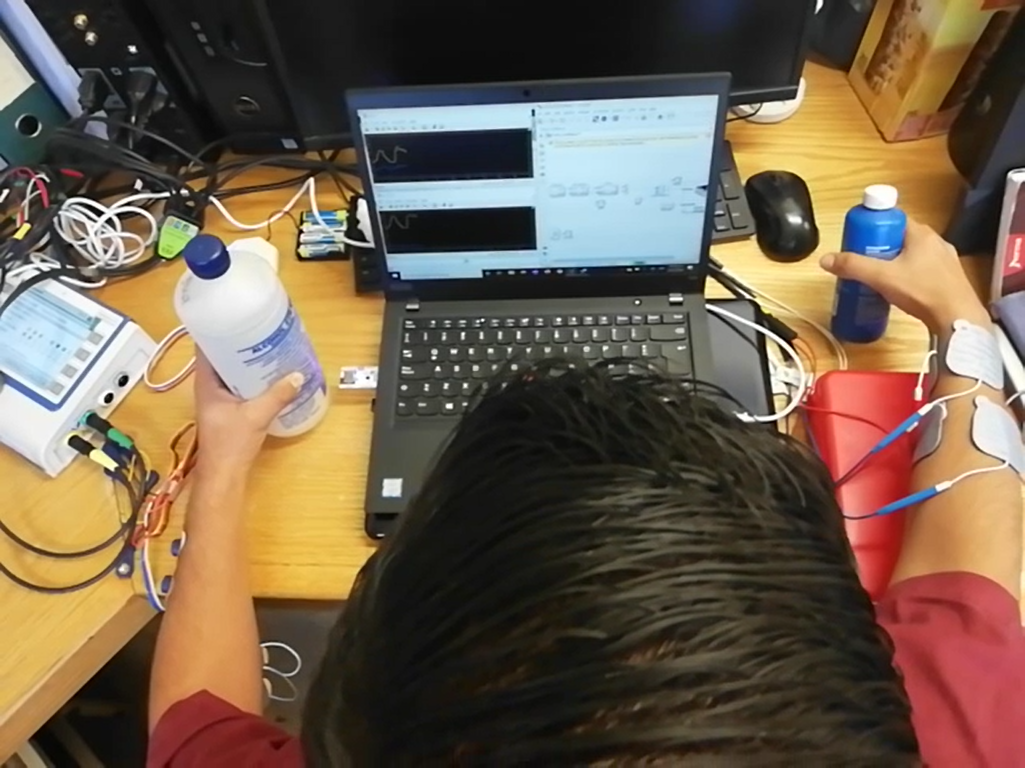
\includegraphics[width=\textwidth]{Funcional_e.png}
		\caption{}
		\label{Figura: Fun_E}
	\end{subfigure}
	\begin{subfigure}[htbp]{0.45\textwidth}
		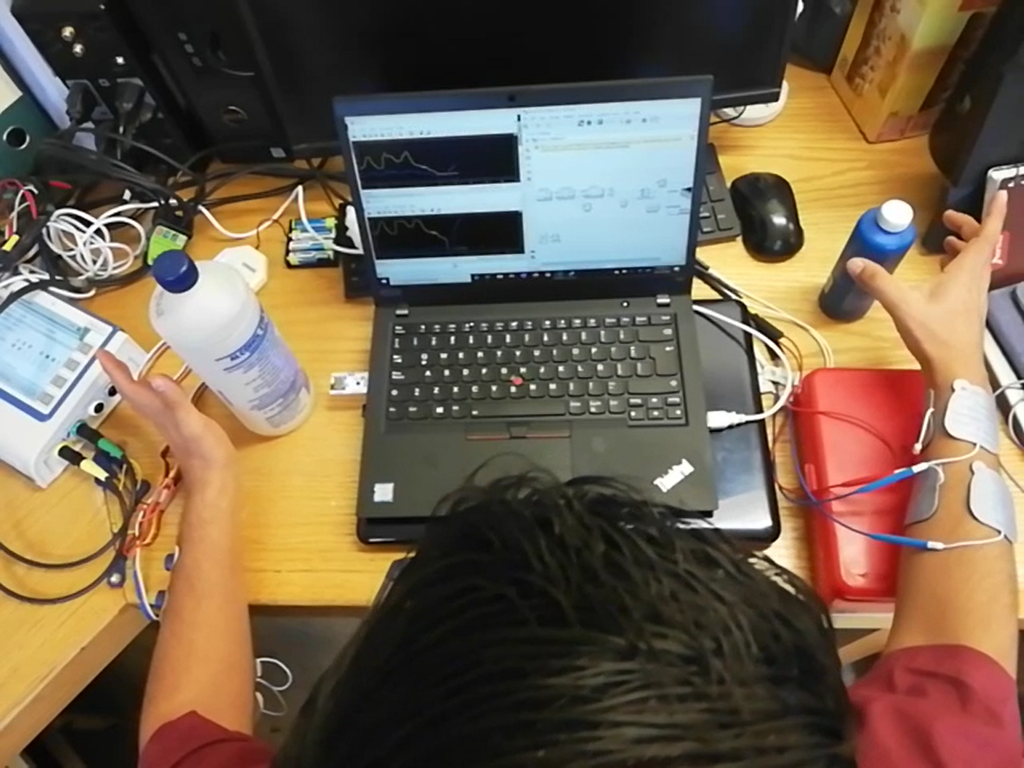
\includegraphics[width=\textwidth]{Funcional_f.png}
		\caption{}
		\label{Figura: Fun_F}
	\end{subfigure}
	\caption[Fases de la tarea funcional asíncrona ejecutada por el sujeto (en línea)]{Fases de la tarea funcional asíncrona ejecutada por el sujeto (en línea). (a)Adducción de hombros. (b)Extensión de dedos. (c)Flexión de dedos. (d)Abducción y extensión de hombros. (e)Flexión de hombros. (f) Extensión de dedos.}
	\label{Figura: TareaFuncional}
\end{figure}

%Figura señales levantar objetos
\begin{figure}[htbp]
	\centering
	\begin{subfigure}[htbp]{0.35\textwidth}
		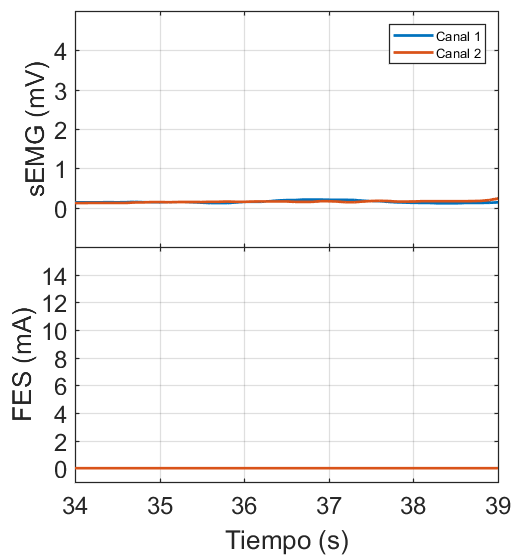
\includegraphics[width=\textwidth]{sEMG_FES_FUN_a.png}
		\caption{}
		\label{Figura: Fun_Sen_A}
	\end{subfigure}
	\hspace*{1cm}
	\begin{subfigure}[htbp]{0.35\textwidth}
		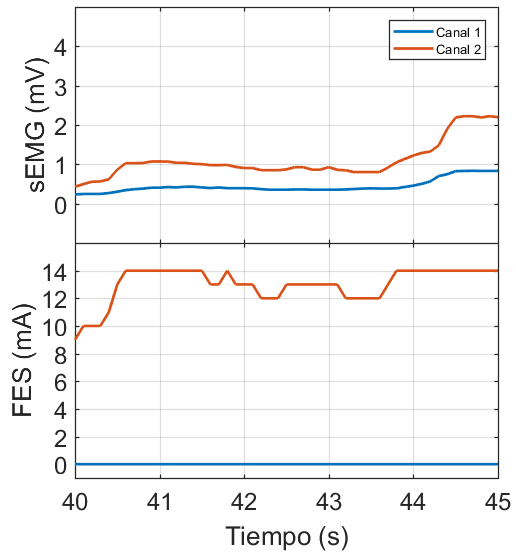
\includegraphics[width=\textwidth]{sEMG_FES_FUN_b.png}
		\caption{}
		\label{Figura: Fun_Sen_B}
	\end{subfigure}
	\newline
	\begin{subfigure}[htbp]{0.35\textwidth}
		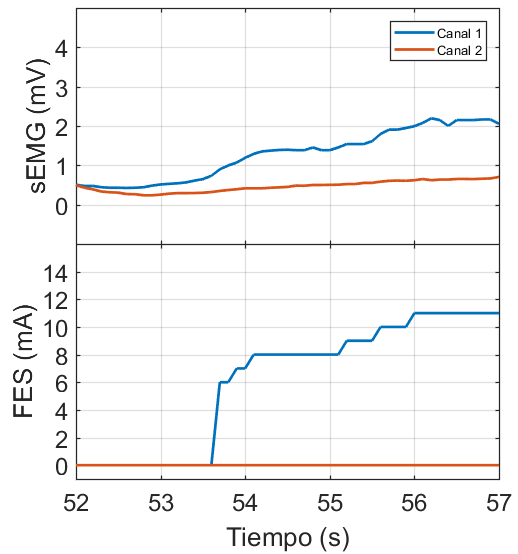
\includegraphics[width=\textwidth]{sEMG_FES_FUN_c.png}
		\caption{}
		\label{Figura: Fun_Sen_C}
	\end{subfigure}
	\hspace*{1cm}
	\begin{subfigure}[htbp]{0.35\textwidth}
		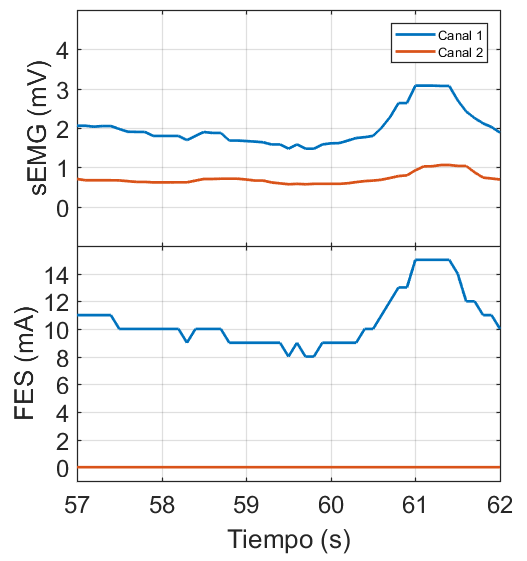
\includegraphics[width=\textwidth]{sEMG_FES_FUN_d.png}
		\caption{}
		\label{Figura: Fun_Sen_D}
	\end{subfigure}
	\newline
	\begin{subfigure}[htbp]{0.35\textwidth}
		\includegraphics[width=\textwidth]{sEMG_FES_FUN_e.png}
		\caption{}
		\label{Figura: Fun_Sen_E}
	\end{subfigure}
	\hspace*{1cm}
	\begin{subfigure}[htbp]{0.35\textwidth}
		\includegraphics[width=\textwidth]{sEMG_FES_FUN_f.png}
		\caption{}
		\label{Figura: Fun_F}
	\end{subfigure}
	\caption[Señales de las fases de la tarea funcional asíncrona ejecutada por el sujeto (en línea)]{Señales de las fases de la tarea funcional asíncrona ejecutada por el sujeto (en línea). Arriba: Señales de sEMG. Abajo: Señales de amplitud FES. Azul: Señales del canal 1. Rojo: Señales del canal 2. (a)Adducción de hombros. (b)Extensión de dedos. (c)Flexión de dedos. (d)Abducción y extensión de hombros. (e)Flexión de hombros. (f) Extensión de dedos.}
	\label{Figura: TareaFuncional_Senales}
\end{figure}


\chapter{Discusión y conclusiones}
%DISCUSIÓN
Este proyecto plantea las bases para implementar una aplicación de estimulación eléctrica en lazo cerrado de miembro superior, a partir de señales sEMG del miembro no afectado en pacientes con hemiplejia por ACV (Accidente Cerebro-Vascular). Los principales resultados obtenidos se discuten en las siguientes secciones, junto a las limitaciones del trabajo y posibles temas para trabajar a futuro. Se espera que el trabajo realizado en este proyecto sea tomado en cuenta para generar mejores técnicas para rehabilitación de pacientes con discapacidad de miembro superior, aplicando dichas técnicas en una neuroprótesis para rehabilitación basada en FES.

\subsubsection*{Adquisición y decodificación de datos}
El subsistema diseñado para realizar la adquisición y decodificación de datos tiene la particularidad de que puede ser utilizado para cualquier dispositivo de adquisición que utilice un chip ADS1299. Tal es el caso del prototipo de adquisición en desarrollo en la División de Investigación Médica del INR-LGII, donde sólo son necesarios pequeños cambios en la selección de los bytes correspondientes a cada canal. Una limitación de este subsistema se encuentra en el bloque responsable de realizar la solicitud de muestras al dispositivo de adquisición, ya que es un bloque perteneciente al \emph{Instrument Control Toolbox} de Simulink\textregistered, por lo cual si no se cuenta con dicho toolbox el sistema no será funcional.

Una posible mejora a este subsistema sería el diseño de un bloque responsable de la solicitud de muestras implementado en algún lenguaje de bajo nivel, esto podría hacer al sistema flexible y veloz, ya que actualmente el bloque de solicitud realiza una comunicación con MATLAB\textregistered \; para poder establecer una conexión serial con el dispositivo de adquisición, proceso que puede estar generando algún retraso dentro de todo el sistema. Un aspecto importante que podría ayudar a rastrear el origen del retardo existente actualmente en el sistema desarrollado en este proyecto, es la medición del retardo que genera dicho subsistema por sí solo, esto podría ayudar a determinar los puntos de trabajo para una versión mejorada.

\subsubsection*{Protocolo para registro de sEMG}
El desempeño del protocolo descrito en este proyecto puede ser afectado por errores humanos al momento de ubicar el lugar adecuado para la colocación de electrodos, por lo cual no se garantiza al 100\% una repetibilidad en los registros. Se propone realizar un estudio donde se analice la actividad mioeléctrica en distintas posiciones del brazo en diversos sujetos, buscando obtener una estandarización en el posicionamiento de electrodos para aplicaciones similares a la desarrollada en este proyecto. Tomar en cuenta para dicho estudio las guías del SENIAM (Surface ElectroMyoGraphy for the Non-Invasive Assessment of Muscles) también puede ayudar a mejorar la repetibilidad en los registros.

\subsubsection*{Procesamiento de sEMG}
Actualmente todo el procesamiento de las señales de sEMG se lleva a cabo por ventanas no traslapadas de adquisición. Este proceso genera un retardo natural definido por la longitud de la ventana analizada, por lo cual el realizar un procesamiento con ventanas traslapadas o bien muestra a muestra podría disminuir este retardo natural. Por otra parte, la implementación de un filtro de mediana móvil resultó de gran utilidad para conseguir una envolvente suave que sirviera como señal de control, sin embargo existen métodos como la regla trapezoidal que podrían arrojar resultados similares, por lo cual se podrían implementar algún otro método y determinar si disminuye el retardo del sistema.

Un aspecto sumamente importante en el procesamiento es el hecho de que no utilizó método alguno de normalización de las señales sEMG. Esto podría estar afectando al desempeño del sistema y sería una buena idea implementar una aplicación similar evaluando el desempeño utilizando sEMG normalizado y no normalizado. Esto último es particularmente importante, ya que la actividad mioeléctrica que presenta un sujeto en diversas sesiones puede cambiar de manera significativa, y claramente la actividad mioeléctrica tampoco será similiar entre diferentes sujetos, por lo que implementar el sistema utilizando señales de sEMG normalizado podría ayudar a estandarizar el sistema de control diseñado.

\subsubsection*{Sistema de control}
Recordando que el sistema de control sEMG-FES consta de dos grandes partes: 1)Máquina de estados finitos para la identificación de movimientos; 2)Control proporcional para modulación sEMG-FES. Se puede comentar lo siguiente:

En cuanto a la identificación de movimientos, se considera que la implementación de un clasificador basado en una FSM que cambia de estado según se superen determinados valores de umbrales no es la mejor forma para realizar una clasificación, pero quizás sí una de las más fáciles. Este clasificador demostró ciertos problemas en identificar cambios de estado que eran notables incluso a simple vista, por ejemplo, en los movimientos incompletos de apertura o cierre existían momentos en los cuales el clasificador no identificaba el movimiento de forma adecuada a pesar de que visualmente se notara un cambio en la envolvente. Además, existe la posibilidad de que los valores de los mismos umbrales puedan estar generando un retardo en el tiempo de inicio de la estimulación eléctrica, ya que habrá movimientos incompletos que no logren pasar ese umbral, y por lo tanto no activar la estimulación eléctrica; una buena idea sería probar disminuir los umbrales para lograr la activación de la estimulación con movimientos ligeros, posiblemente acompañados de otros algoritmos de procesamiento. Otro aspecto importante de este clasificador, es la imposibilidad de compensar la fatiga muscular. Implementar un clasificador robusto basado en algún algoritmo de inteligencia artificial podría ser de mayor utilidad para una aplicación que considere estos y otros aspectos relevantes para su uso en rehabilitación.

En cuanto al mapeo proporcional encargado de la modulación de la amplitud FES, hay que destacar que este se obtiene a partir de dos umbrales obtenidos en la etapa de calibración, y considerando que el sEMG no presenta un comportamiento lineal, es probable que este método para la obtención de la ecuación del mapeo proporcional no pueda realizar un seguimiento preciso a los cambios existentes en las señales de sEMG. Una mejora a esta parte podría ser la implementación de un procedimiento de calibración con más de dos puntos, y a partir de ellos obtener una regresión lineal, o en su momento introducir algún modelo de control que represente la relación existente entre las señales sEMG y la fuerza ejercida o el torque muscular. Cabe destacar que debido a que la técnica de retroalimentación utilizada para este proyecto es el biofeedback, no existe como tal una señal de retroalimentación como parte del mapeo proporcional, porque no se usa una diferencia entre un setpoit y el valor de una variable de salida. Para que este mapeo fuera realmente un control proporcional, de acuerdo a su definición, la señal de control debería ser una señal de error obtenida a partir de la diferencia entre la señal ideal y la señal real, por ejemplo, la señal de sEMG del miembro no afectado y la señal de sEMG del miembro afectado o el ángulo o rango de movimiento de la muñeca esperado y el medido. El agregar una señal de retroalimentación objetiva que pueda ser considerada dentro del sistema de control probablemente mejorará el desempeño.

Relacionado a las pruebas con la aplicación sEMG-FES contralateral (validación en línea con FES y tarea funcional asíncrona), el hecho de que se lograra llevar a cabo con éxito a pesar de las limitaciones ya mencionadas de los distintos bloques del sistema, es un indicador del potencial que tiene el enfoque propuesto en este proyecto, para el desarrollo de aplicaciones para terapia de rehabilitación, dando a los pacientes la posibilidad de realizar tareas comunes de la vida diaria que serían imposibles de realizar para ellos de otro modo. Se espera que con las correctas adecuaciones, el sistema diseñado en este proyecto pueda ser de utilidad en sujetos con hemiplejia. Adicionalmente, sería bueno realizar una variante de esta prueba donde se llevara a cabo el mismo procedimiento pero mediante un experimento cruzado (un sujeto controla mientras otro sujeto es estimulado), y junto con algún algoritmo de visión por computadora poder determinar el retardo existente en esta prueba, para así tener una métrica más sobre el desempeño del sistema. O bien, introduciendo una señal sintética similar al sEMG que permita la medición exacta de los tiempos de retardo.


\subsubsection*{Conclusiones}
La aplicación sEMG-FES diseñada en este trabajo logró cumplir el objetivo principal del mismo, y además, pese a las limitaciones del sistema, se logró demostrar que el enfoque utilizado en este trabajo puede ser de utilidad en aplicaciones diseñadas para terapia de rehabilitación.

Relacionado al protocolo de registro se concluye que este es susceptible a errores humanos, por lo cuál es recomendable utilizar otro protocolo o seguir guías clínicas como las ya mencionadas guías del SENIAM.

En cuanto al algoritmo para clasificación de movimientos, se destaca que el algoritmo diseñado basado en umbrales fue útil para verificar la viabilidad del sistema sEMG-FES desarrollado, aunque con un desempeño subóptimo. En el futuro se pueden implementar soluciones basadas en algoritmos de inteligencia artificial, que probablemente arrojen mejores resultados.

Por último, relacionado al mapeo sEMG-FES, se obtuvo una solución rápida y sencilla, la cuál se puede adaptar a diferentes tipos de señales con las que se cuente. Sin embargo, al tener el sEMG un comportamiento no lineal es probable que este este método no sea el idóneo para dicha señal, abriendo la posibilidad al uso de otros esquemas de control.


\renewcommand{\bibname}{Referencias}
\bibliographystyle{acm}
\bibliography{7_Bibliografia}

\end{document}